\newpage
\section{Problem5.9}
\subsection{Rosenbrock函数图像}
首先画出Rosenbrock函数的图像及等值线如下\footnote{由于Rosenbrock函数过于陡峭,因此对原函数进行了取对数处理,以便于观察其特点。}:


\begin{figure}[H]
\centering
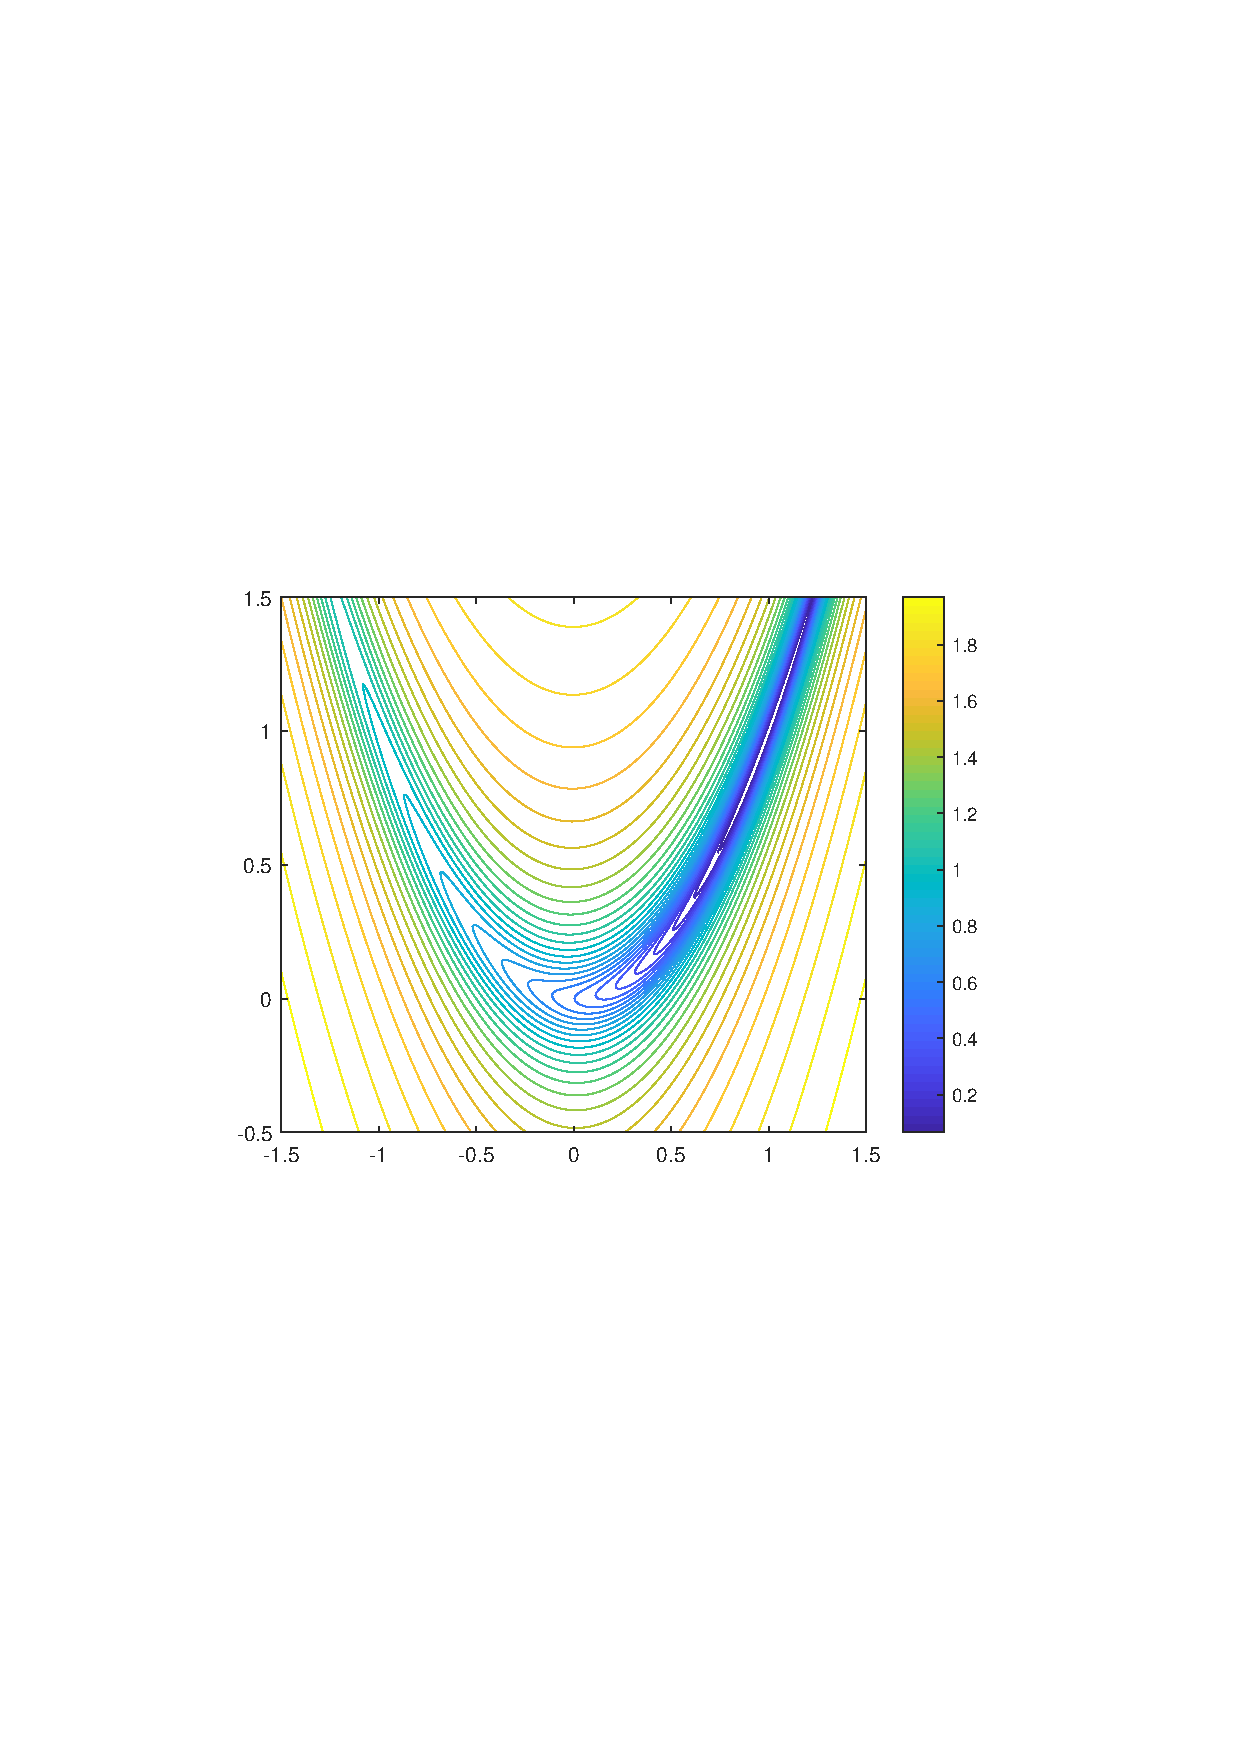
\includegraphics[width=11cm]{fig/4_01.pdf}
\end{figure}


\begin{figure}[H]
\centering
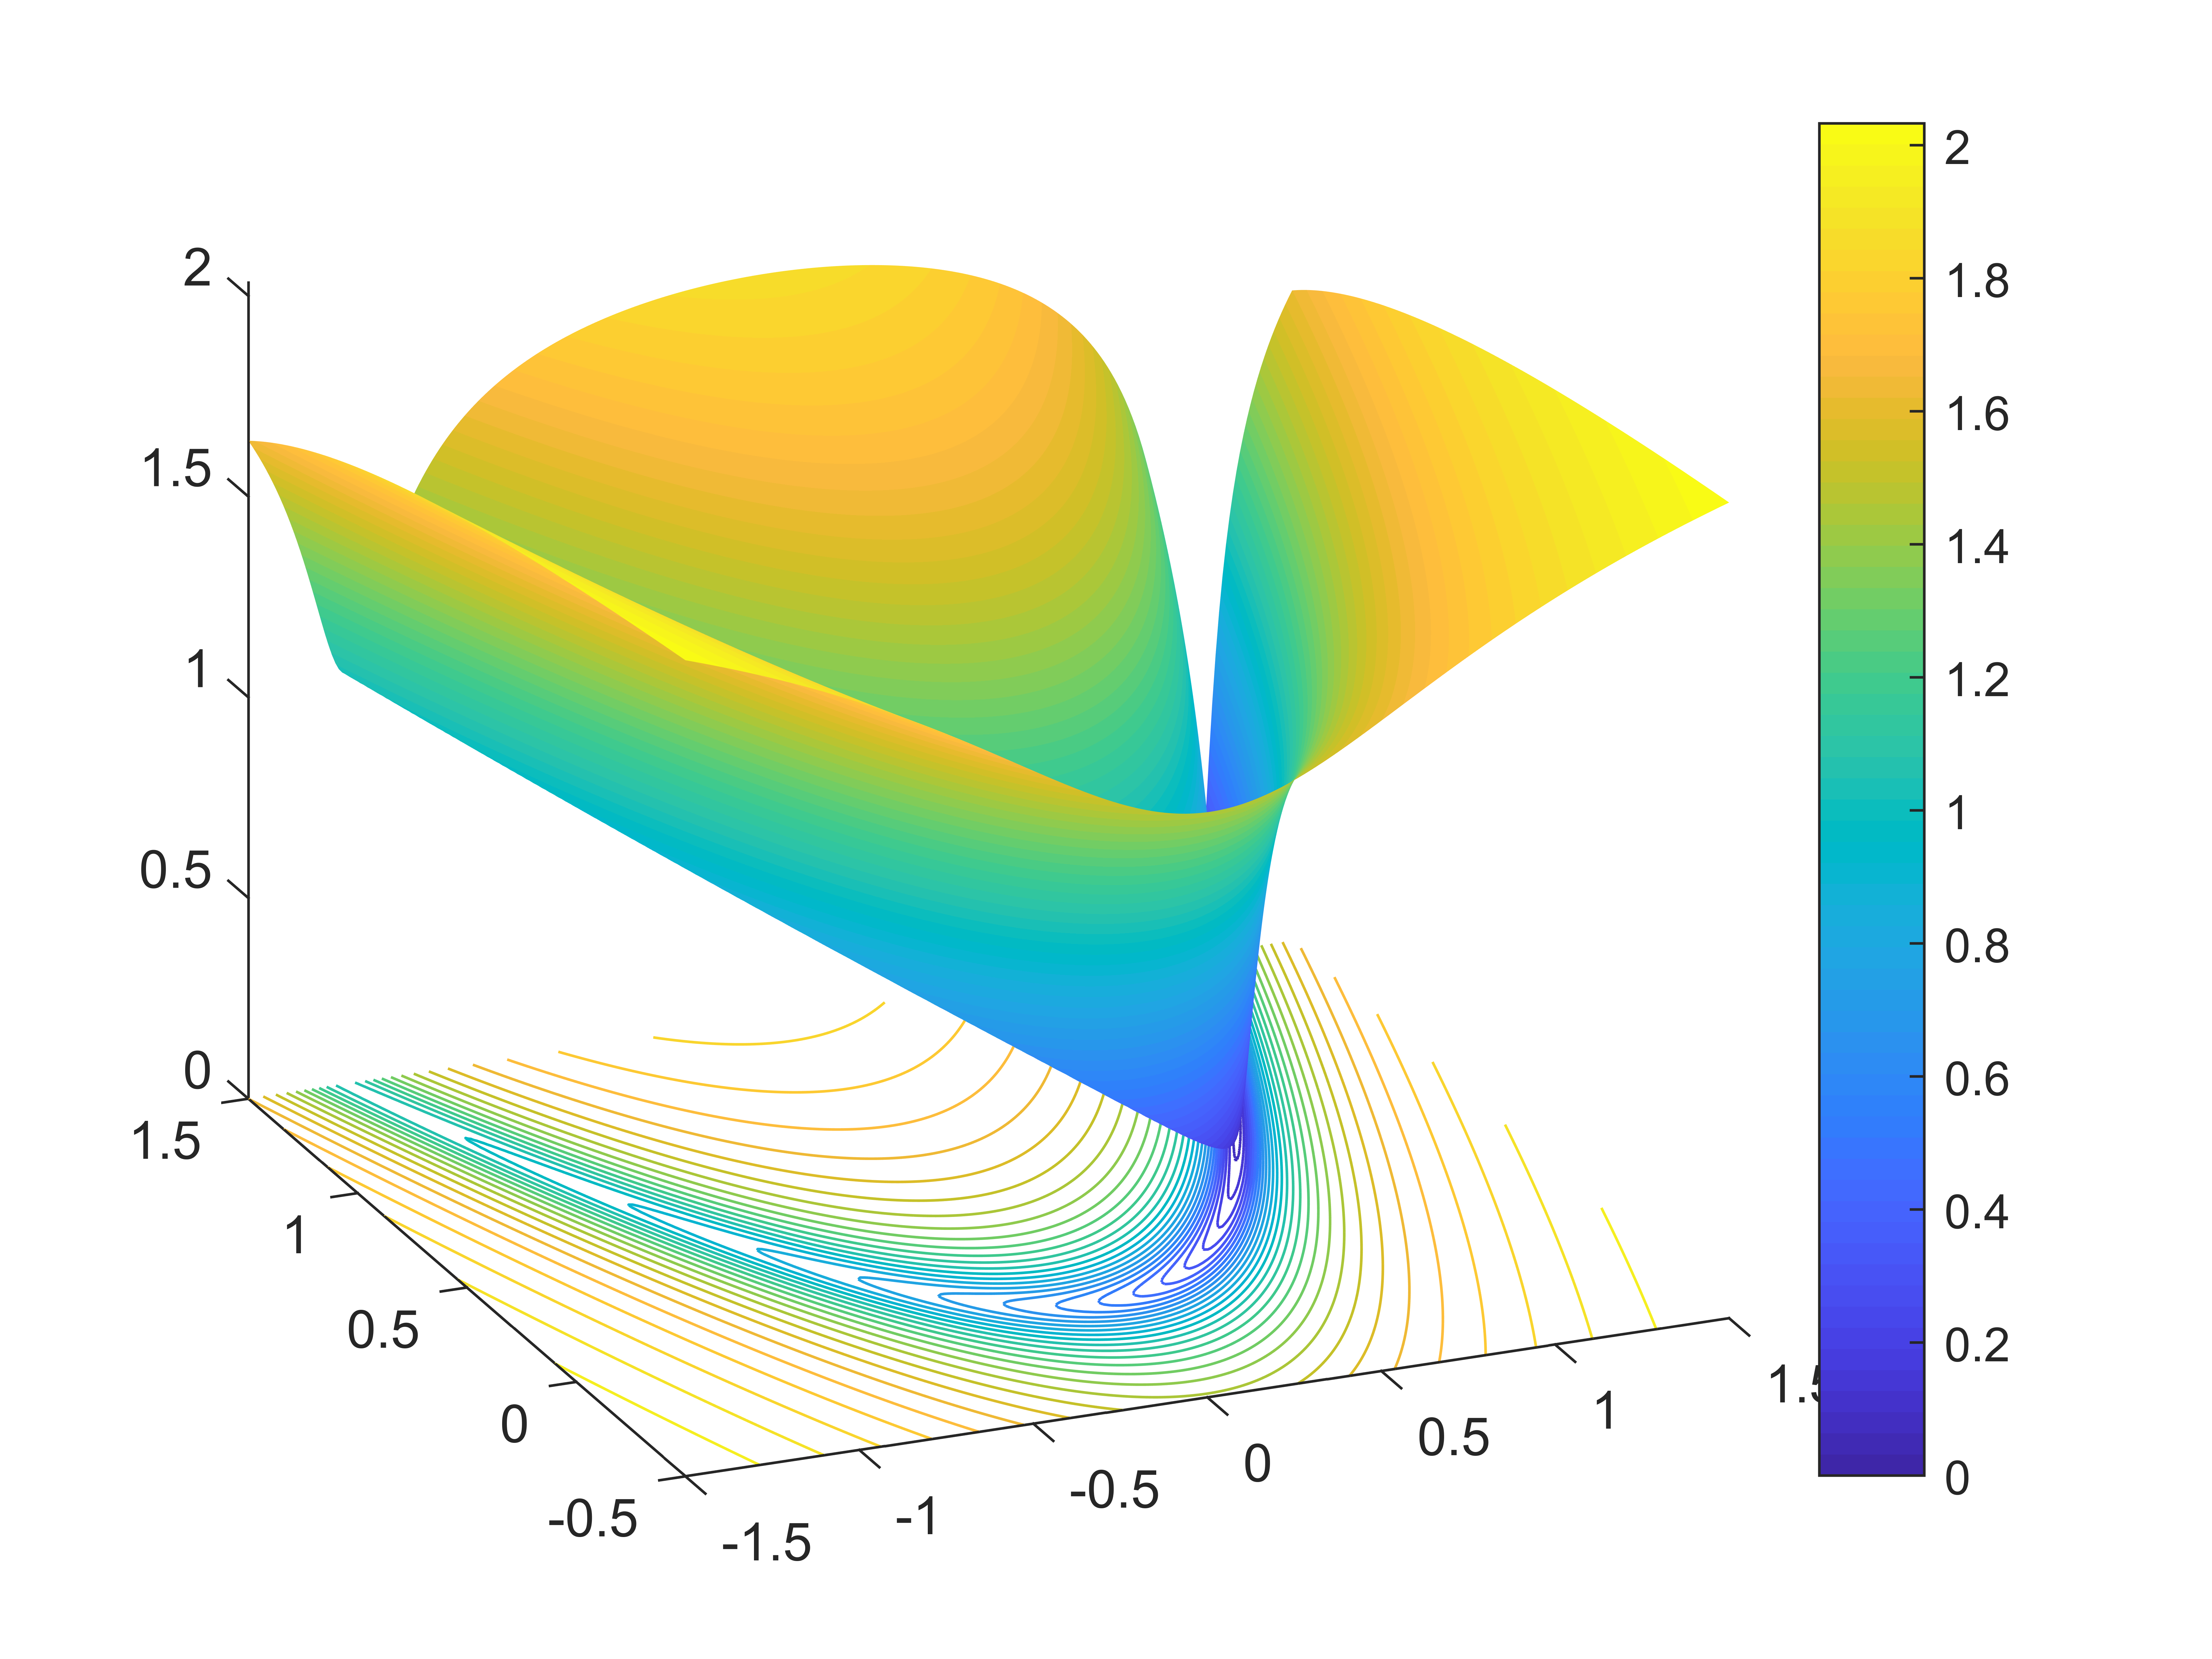
\includegraphics[width=11cm]{fig/4_02.png}
\end{figure}

\subsection{算法伪代码}

\begin{algorithm}[h]  
\caption{Backtracking-Armijo Line Search}  
\begin{algorithmic}[1]  
\STATE Choose $\bar{\alpha}>0,\quad \gamma,\rho\in (0,1)$
\STATE Set $\alpha=\bar{\alpha}$
\WHILE {$\phi(\alpha)>\phi(0)+\rho\phi'(0)\alpha$}
\STATE Set $\alpha=\gamma\alpha$
\ENDWHILE
\RETURN $\alpha$ as $\alpha_k$
\end{algorithmic}  
\end{algorithm}


\begin{algorithm}[h]  
\caption{Steepest-denscent-Armijo method for problem(5.9)}  
\begin{algorithmic}[1]  
\STATE Given $\bm{x}^{(0)}$ and $G$
\STATE Set $\bm{p}^{(0)}=-\bm{g}^{(0)},k=0$
\WHILE {$\|\bm{g}^{(k)}\|>\epsilon$}
\STATE Compute $\alpha_k$ by Backtracking-Armijo Line Search
\STATE Set $\bm{x}^{(k+1)}=\bm{x}^{(k)}+\alpha_k\bm{p}^{(k)}$
\STATE Set $\bm{g}^{(k+1)}=g(\bm{x}^{(k+1)})$
\STATE Set $\bm{p}^{(k)}=-\bm{g}^{(k)}$
\STATE k=k+1
\ENDWHILE
\end{algorithmic}  
\end{algorithm}

\begin{algorithm}[h]  
\caption{Newton-Armijo method for problem(5.9)}  
\begin{algorithmic}[1]  
\STATE Given $\bm{x}^{(0)}$ and compute $\bm{g}(\bm{x})= \nabla f(\bm{x})$
\STATE Compute $\bm{G}(\bm{x})= \nabla {\bm{g}(\bm{x})}^T$
\STATE Set $\bm{g}^{(0)}=\bm{g}(\bm{x}^{(0)}),k=0$
\WHILE {$\|\bm{g}^{(k)}\|_2>\epsilon$}
\STATE Set $\bm{s}^{(k)}=-{\bm{G}^{(k)}}^{-1}\bm{g}^{(k)}$
\STATE Compute $\alpha_k$ by Backtracking-Armijo Line Search
\STATE Set $\bm{x}^{(k+1)}=\bm{x}^{(k)}+\alpha_k\bm{s}^{(k)}$
\STATE Set k=k+1
\ENDWHILE
\end{algorithmic}  
\end{algorithm} 

\subsection{计算结果展示}

本题中Armijo线搜索的参数为$\gamma=0.5,\rho=0.01$,并设置最大搜索步长为200.

然后分别以梯度下降法和牛顿法迭代,并画出等高线、运动轨迹、迭代值如下:

\begin{figure}[H]
\centering
\subfigure{
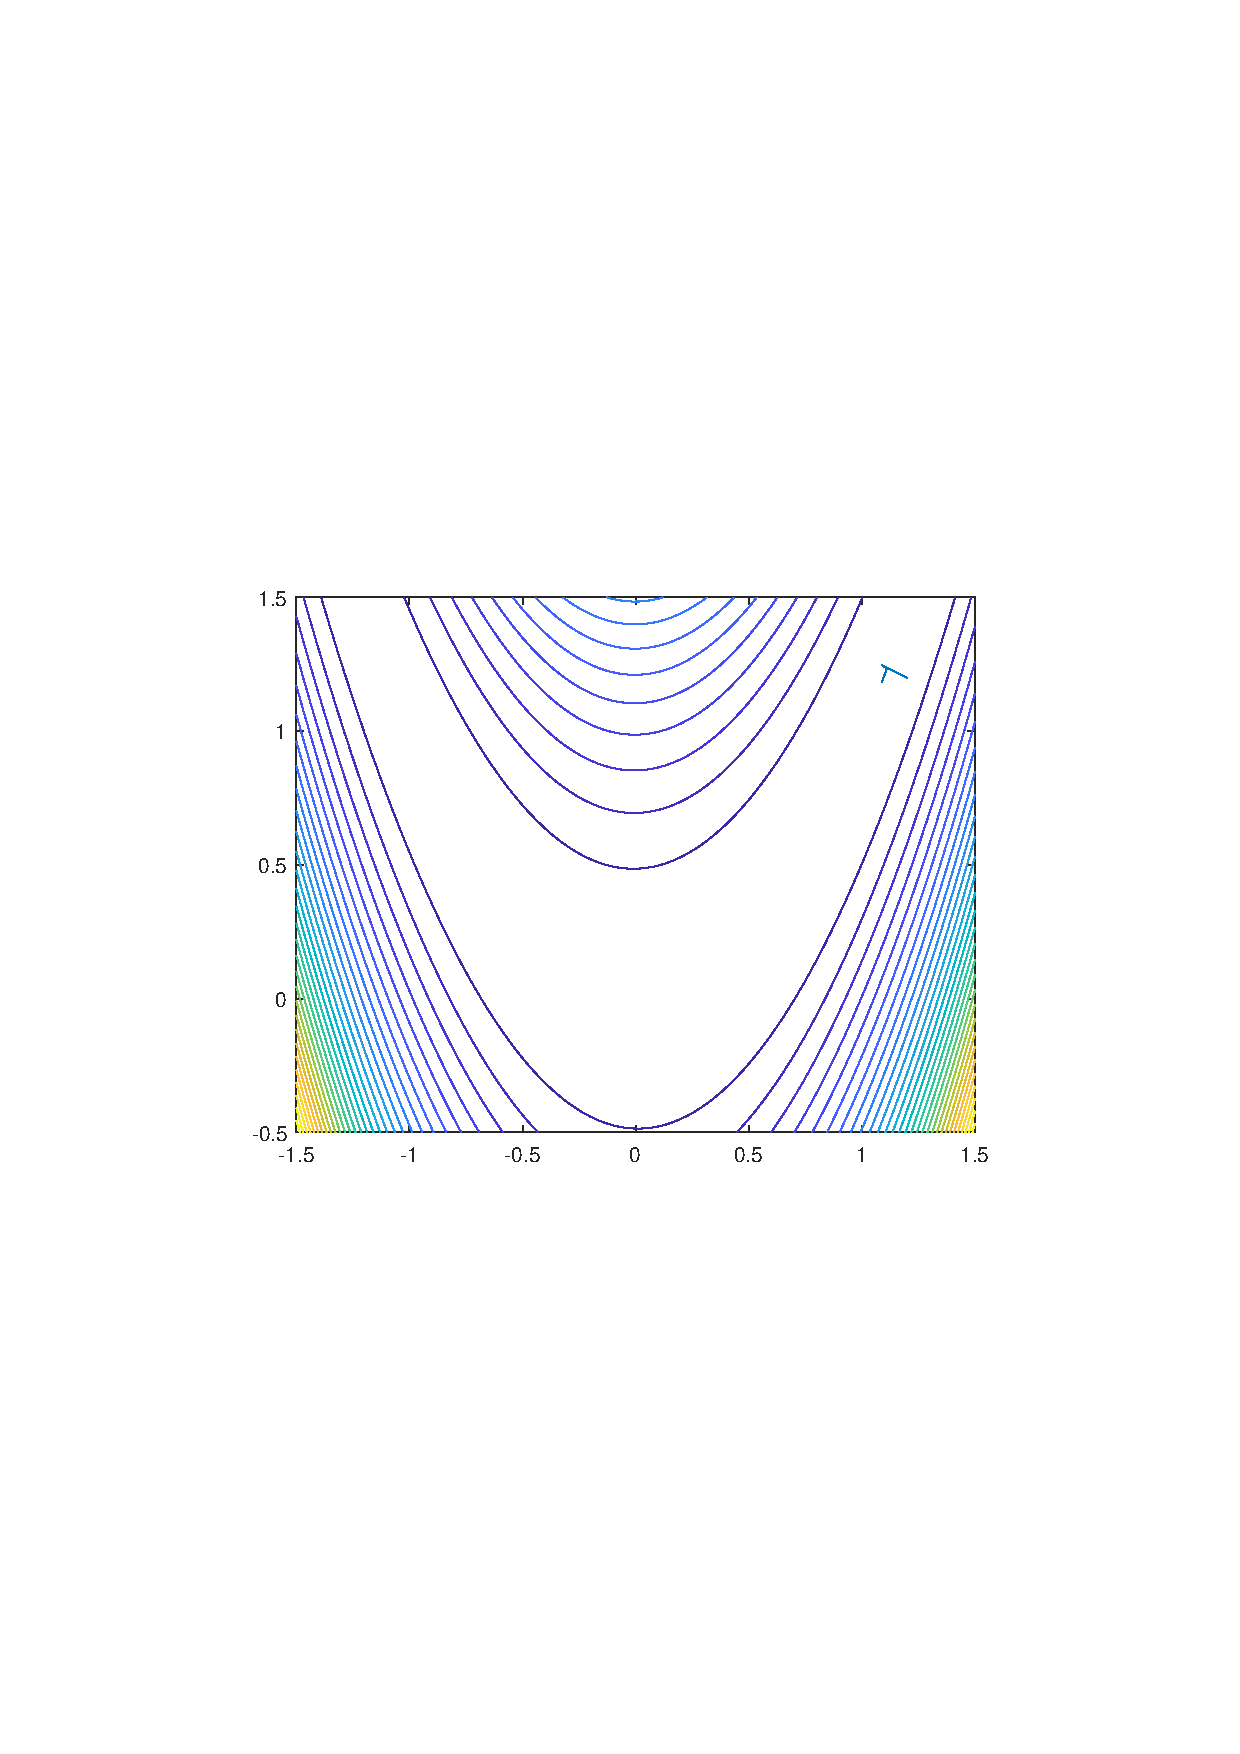
\includegraphics[width=5cm]{fig/4_11.pdf}}
\subfigure{
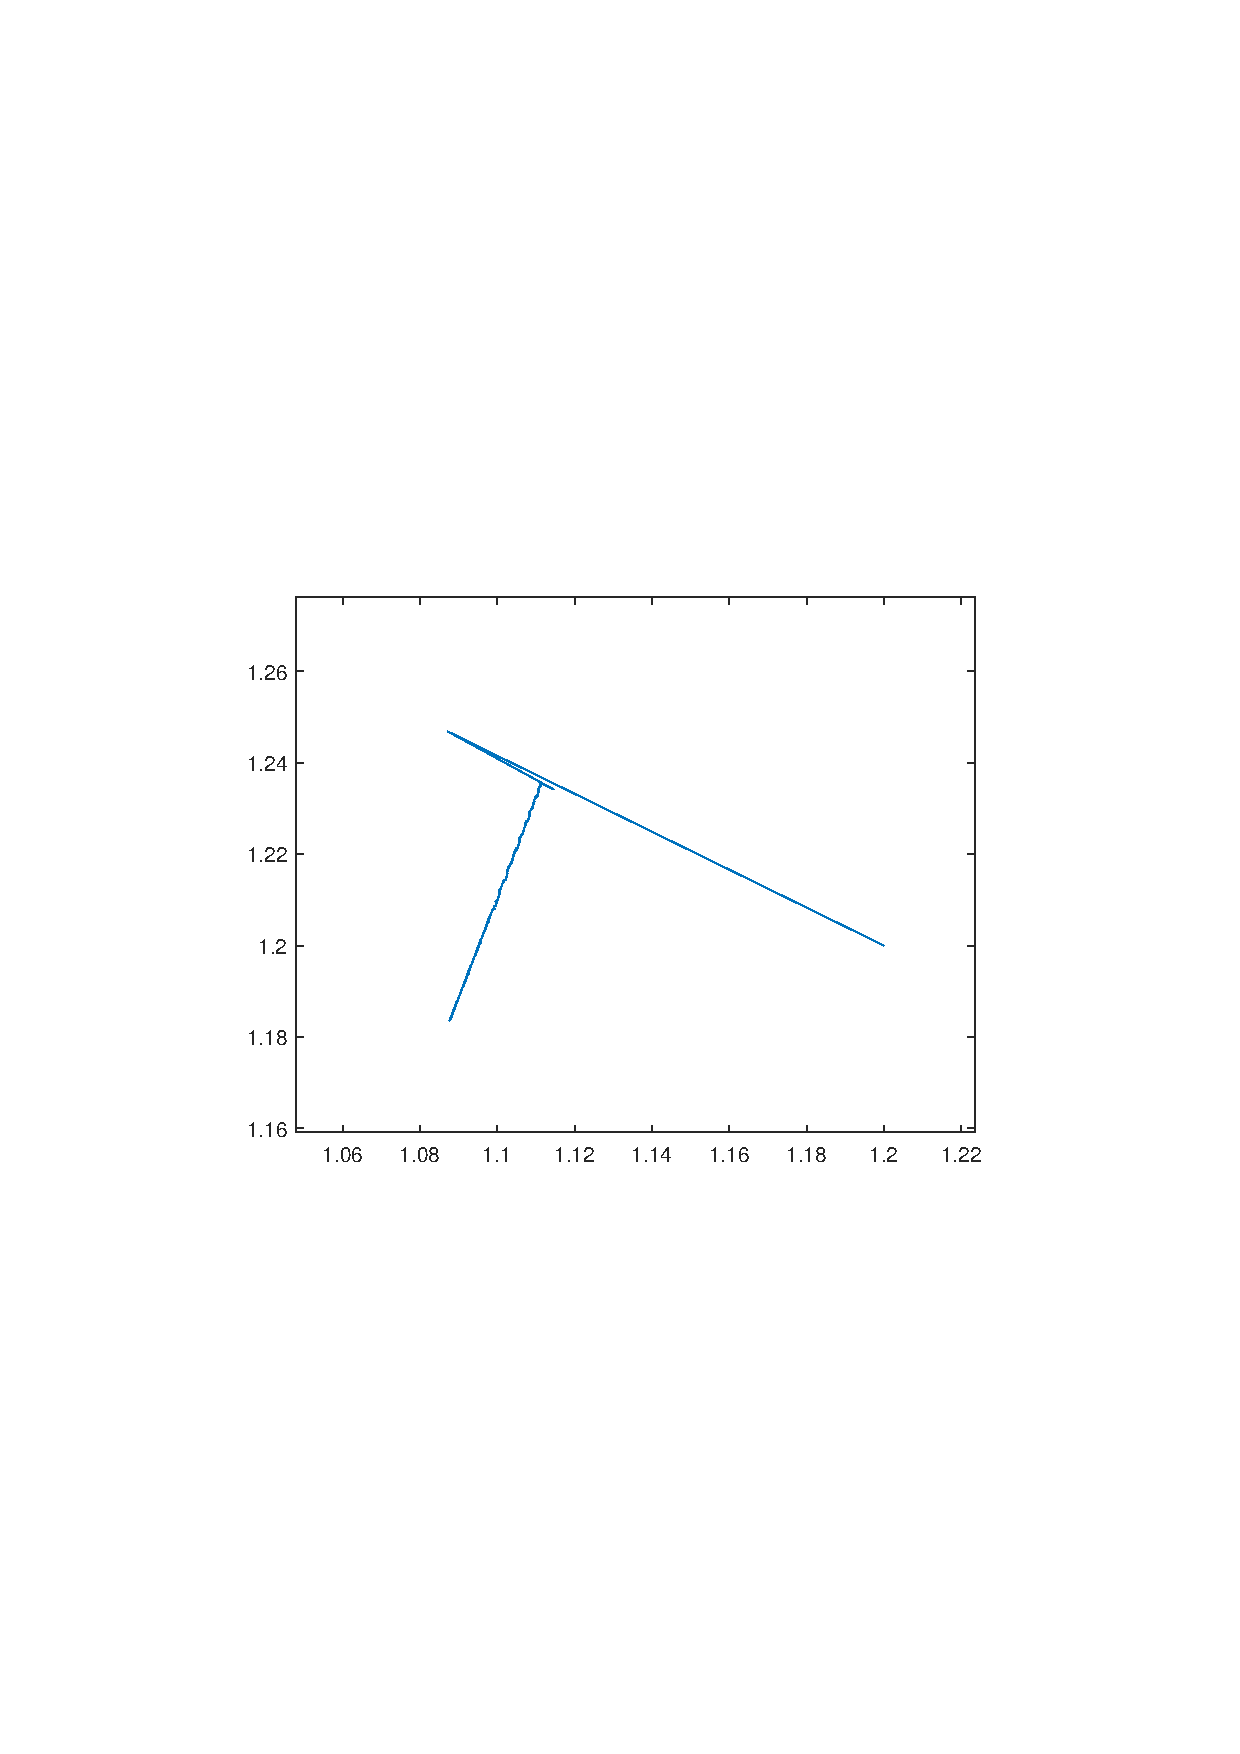
\includegraphics[width=5cm]{fig/4_12.pdf}}
\subfigure{
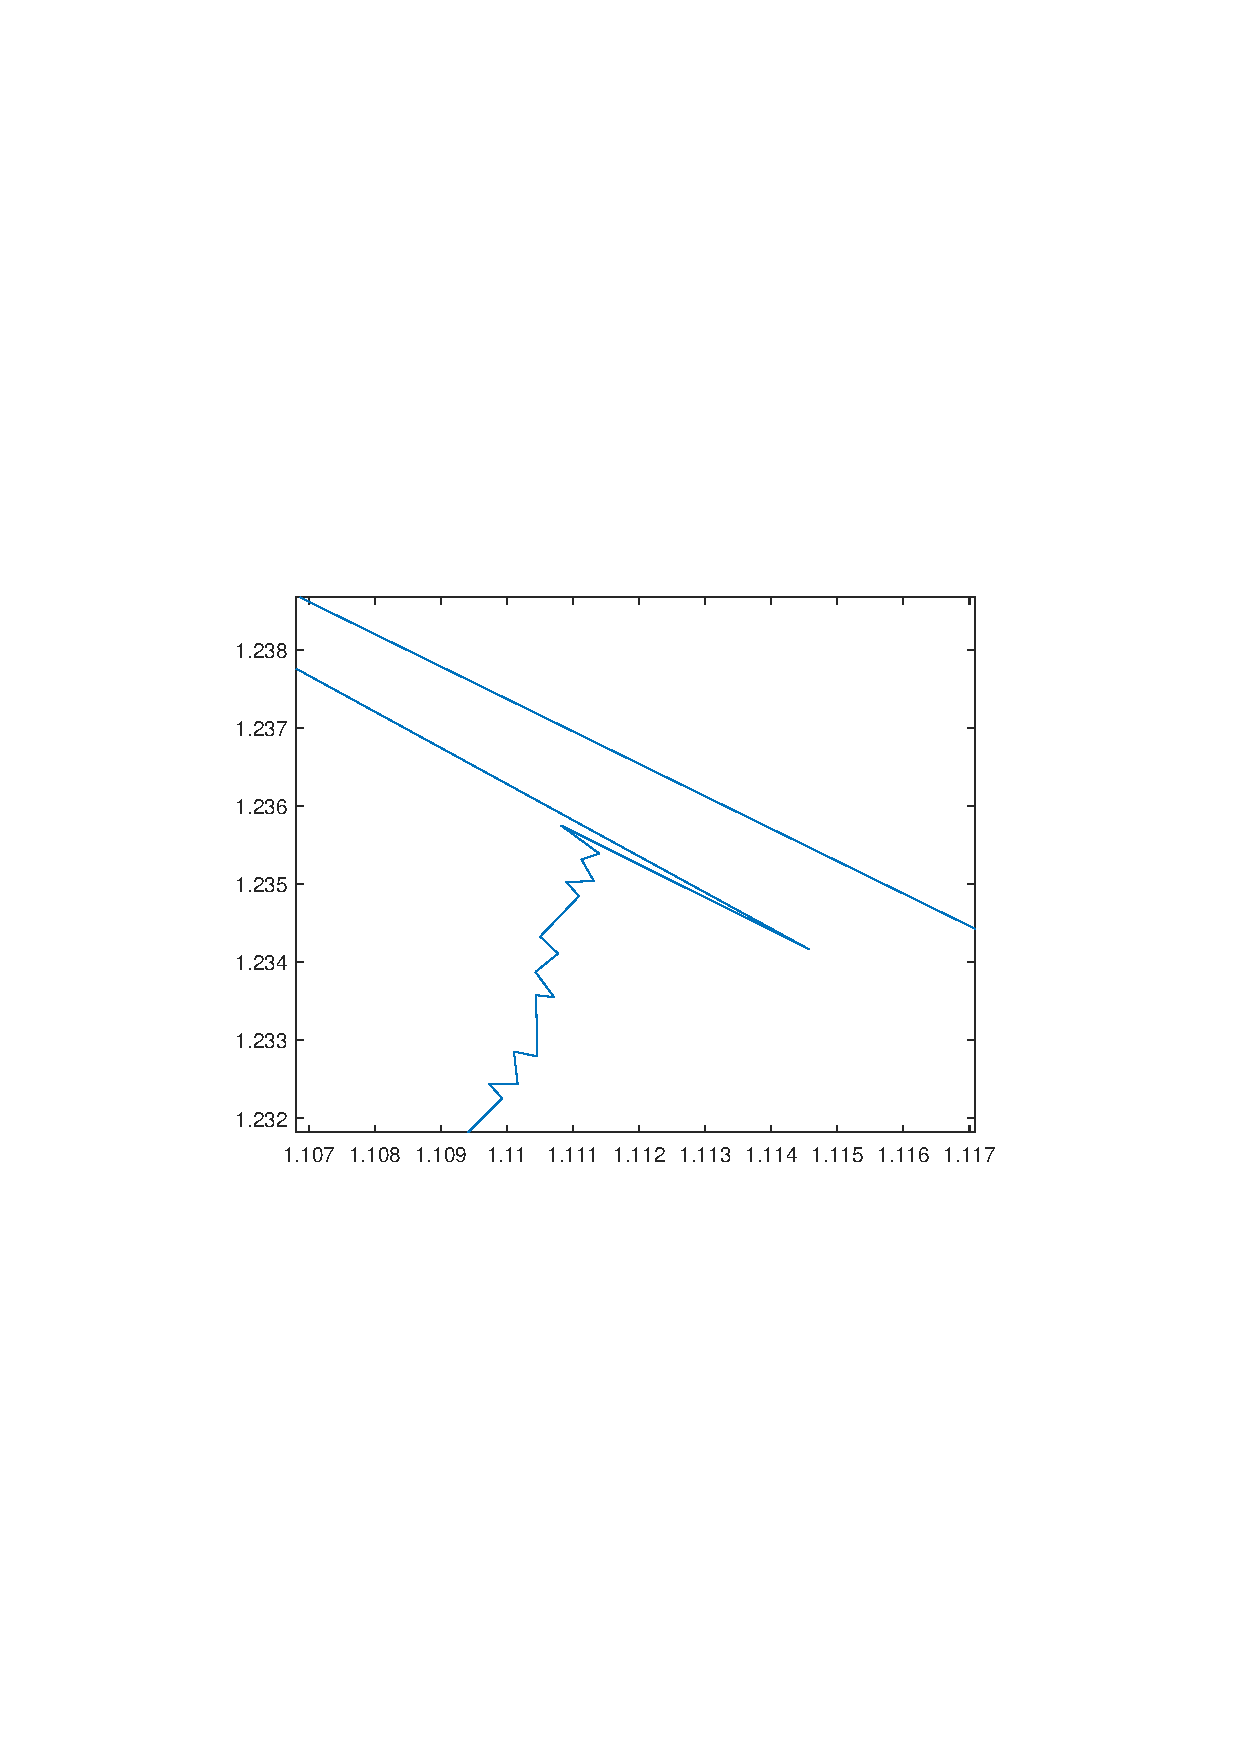
\includegraphics[width=5cm]{fig/4_13.pdf}}
\subfigure{
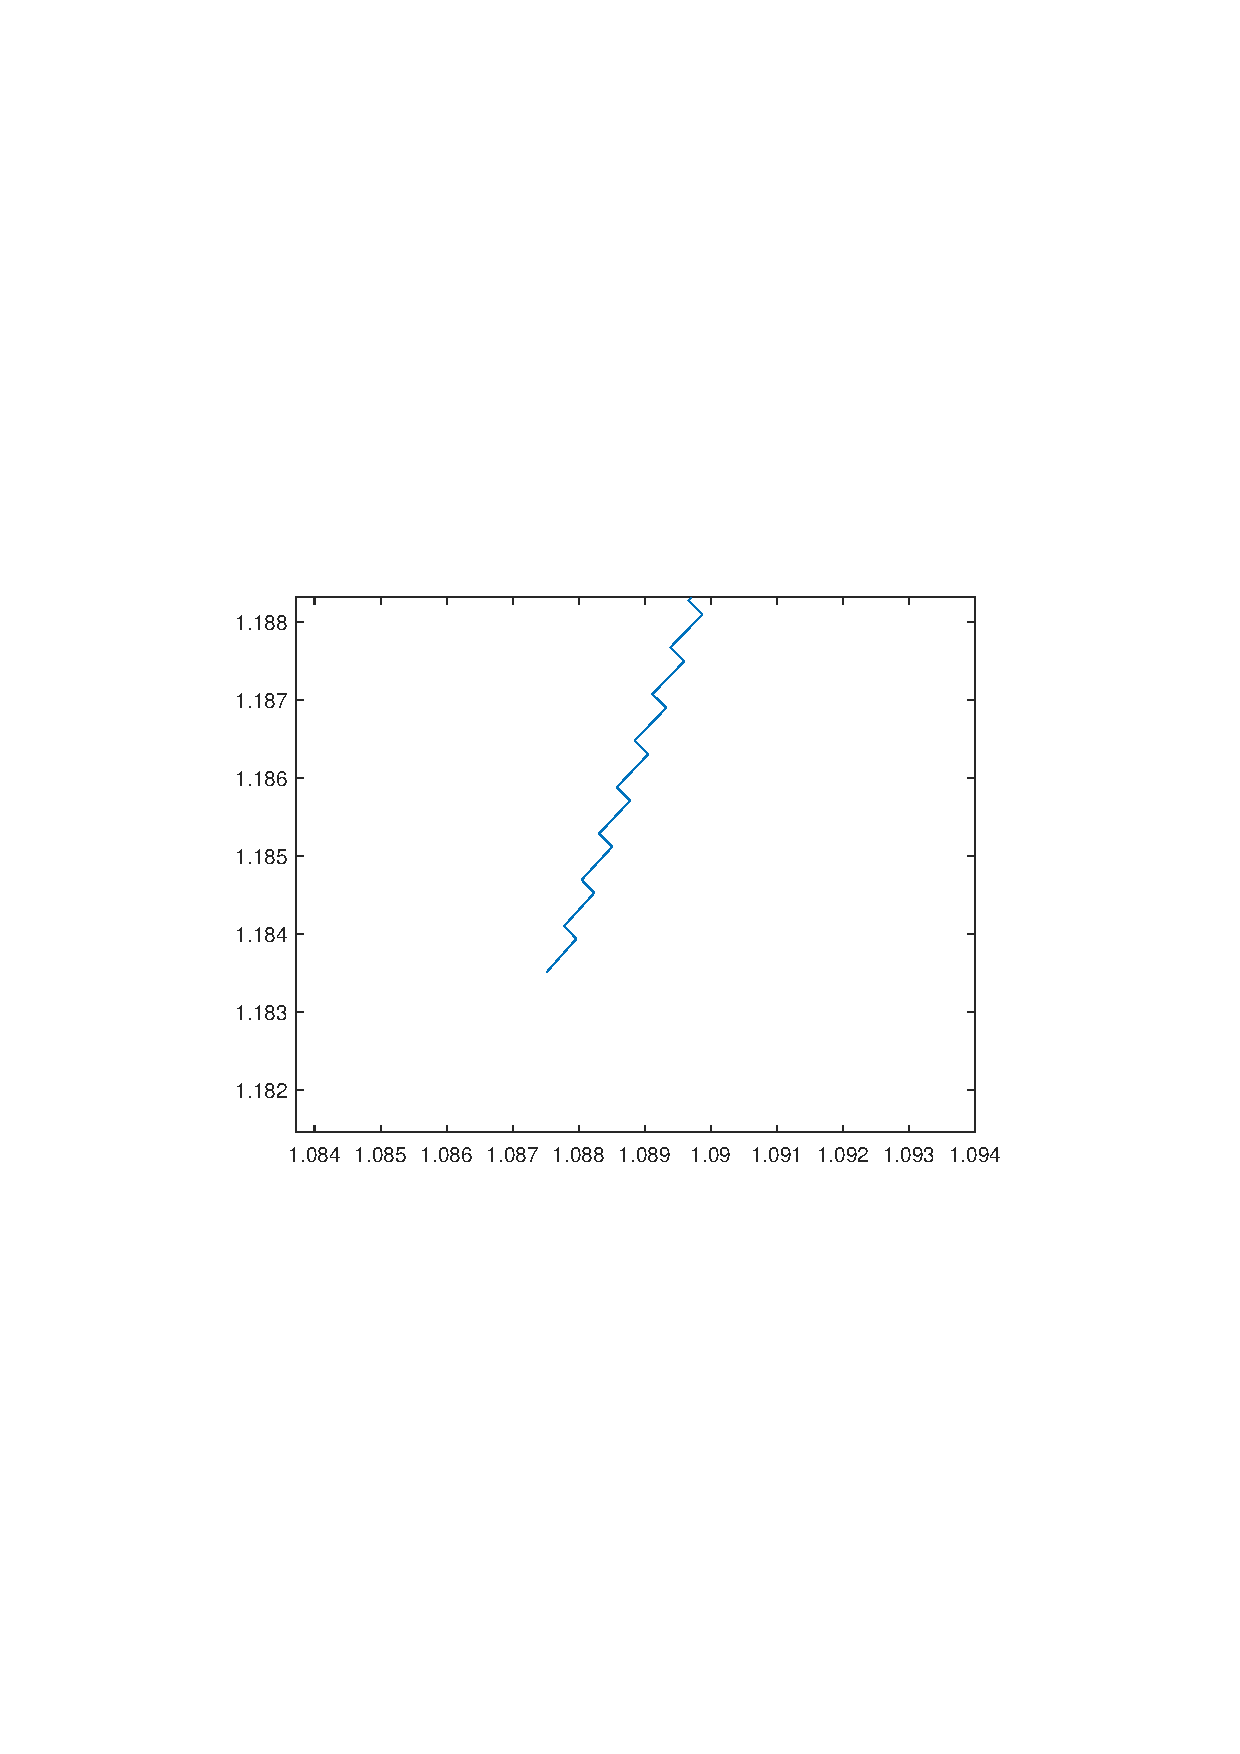
\includegraphics[width=5cm]{fig/4_14.pdf}}
\caption{Steepest-denscent in (1.2,1.2)}
\label{Fig.lable}
\end{figure}

\begin{figure}[H]
\centering
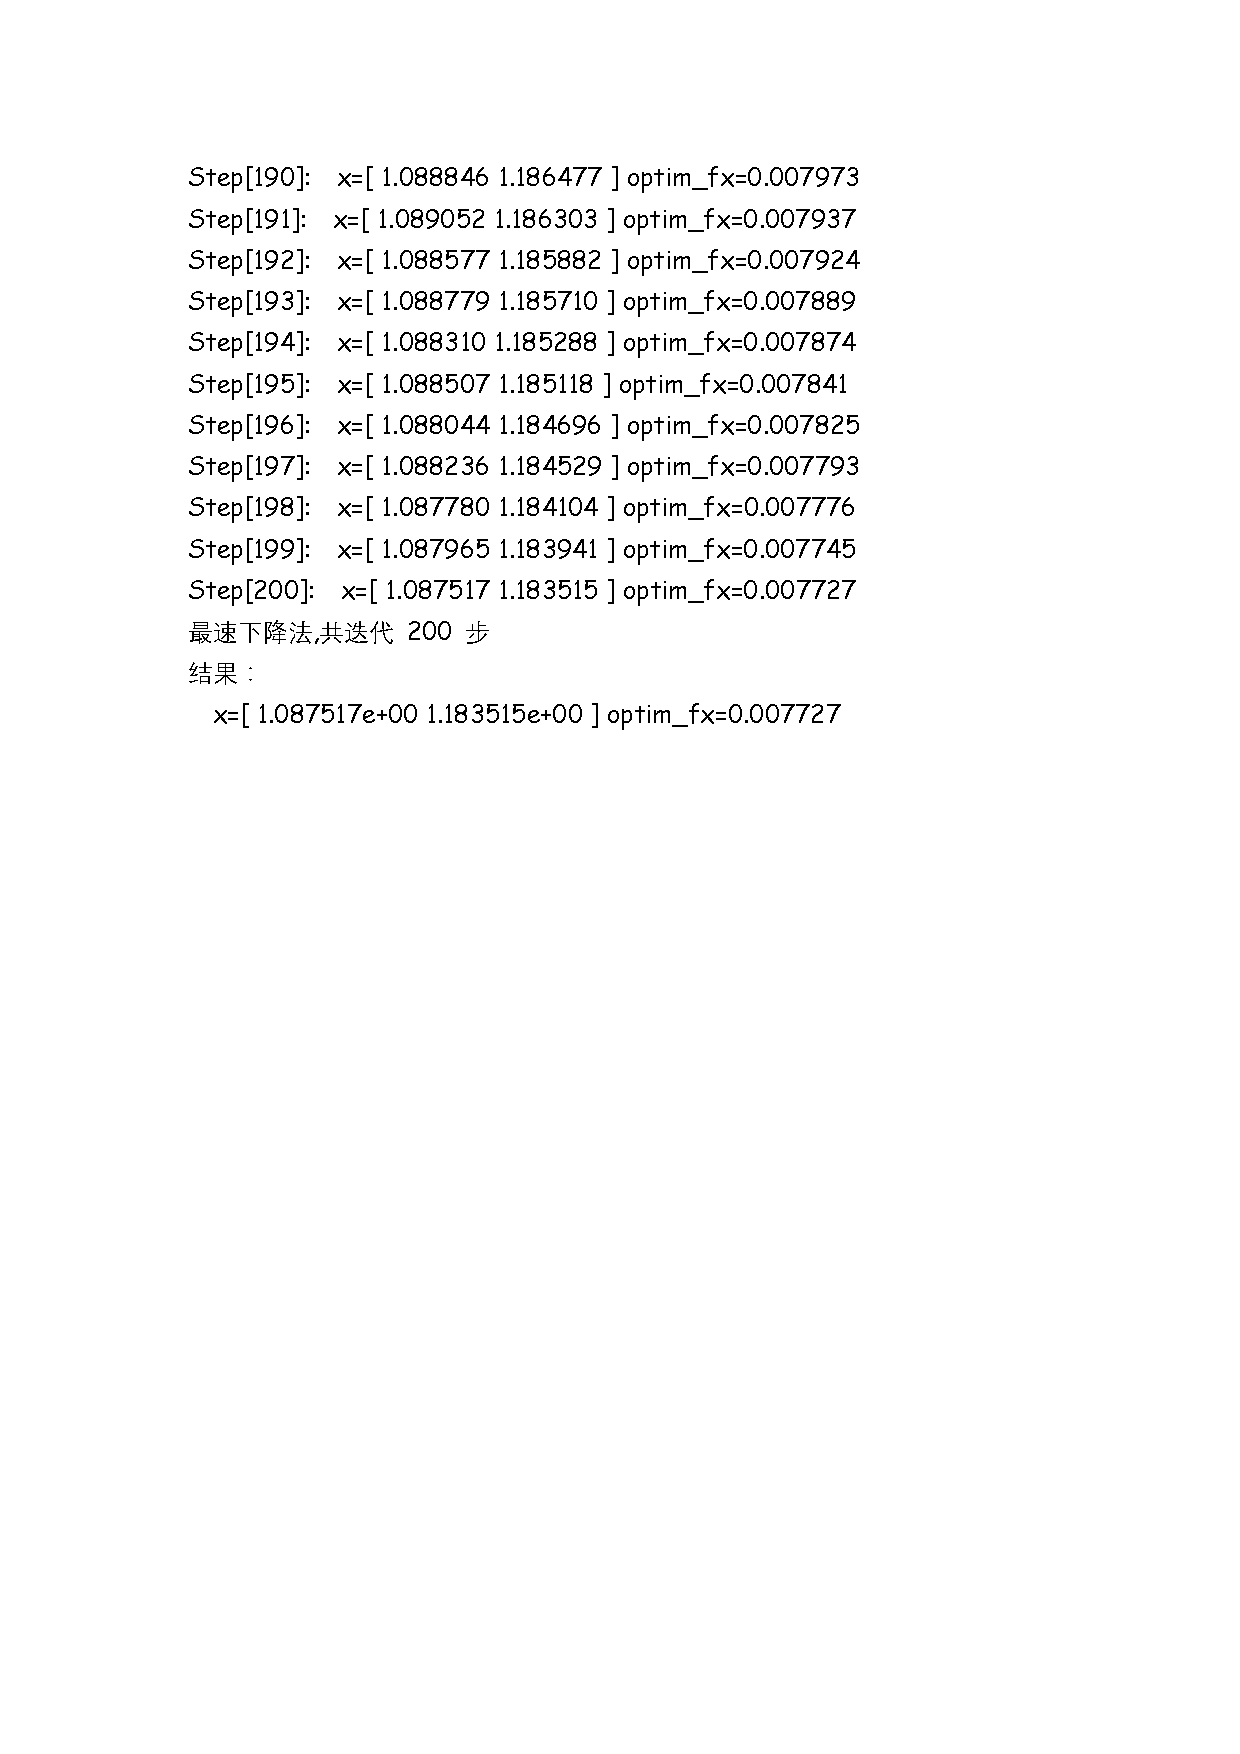
\includegraphics[width=10cm]{fig/4_15.pdf}
%\caption{在$(1,1)$处附近的三维等高线}
\end{figure}

\begin{figure}[H]
\centering
\subfigure{
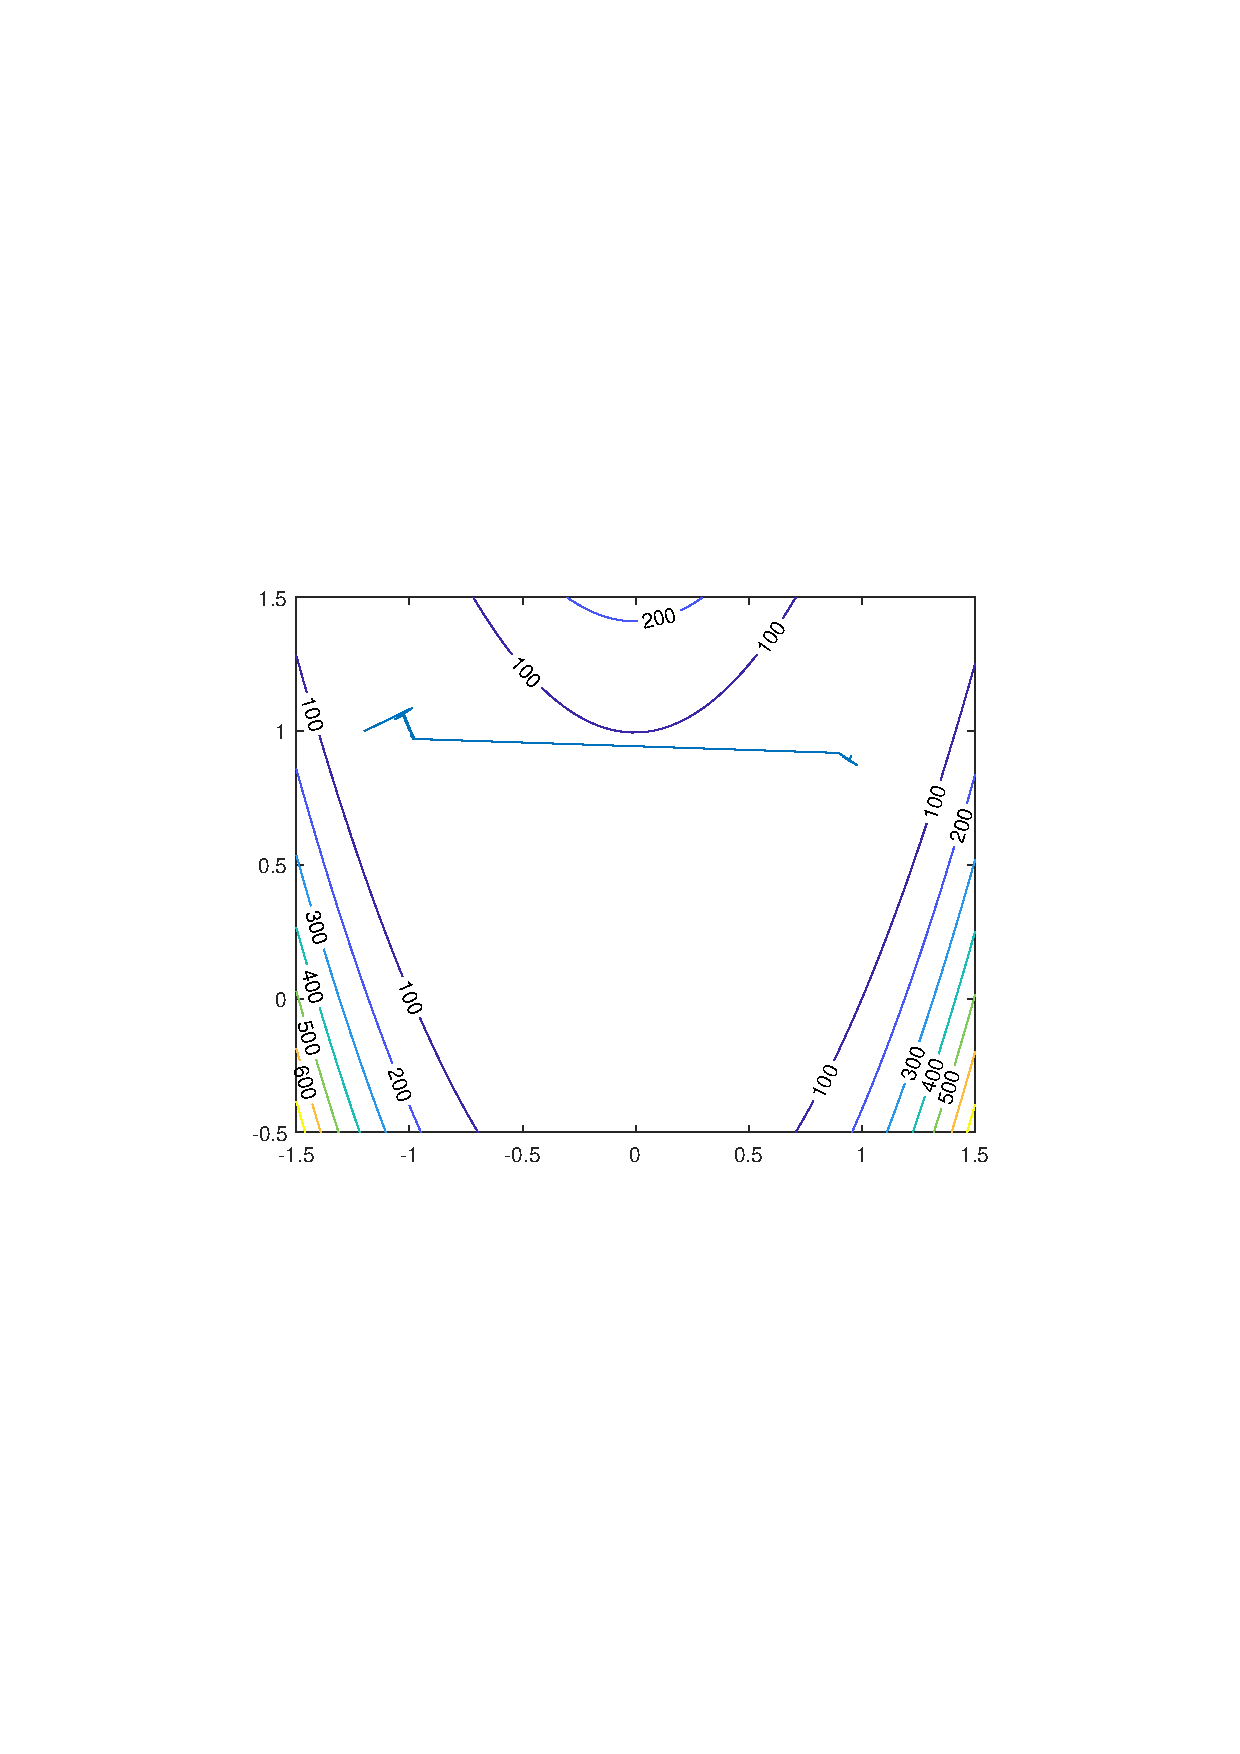
\includegraphics[width=5cm]{fig/4_21.pdf}}
\subfigure{
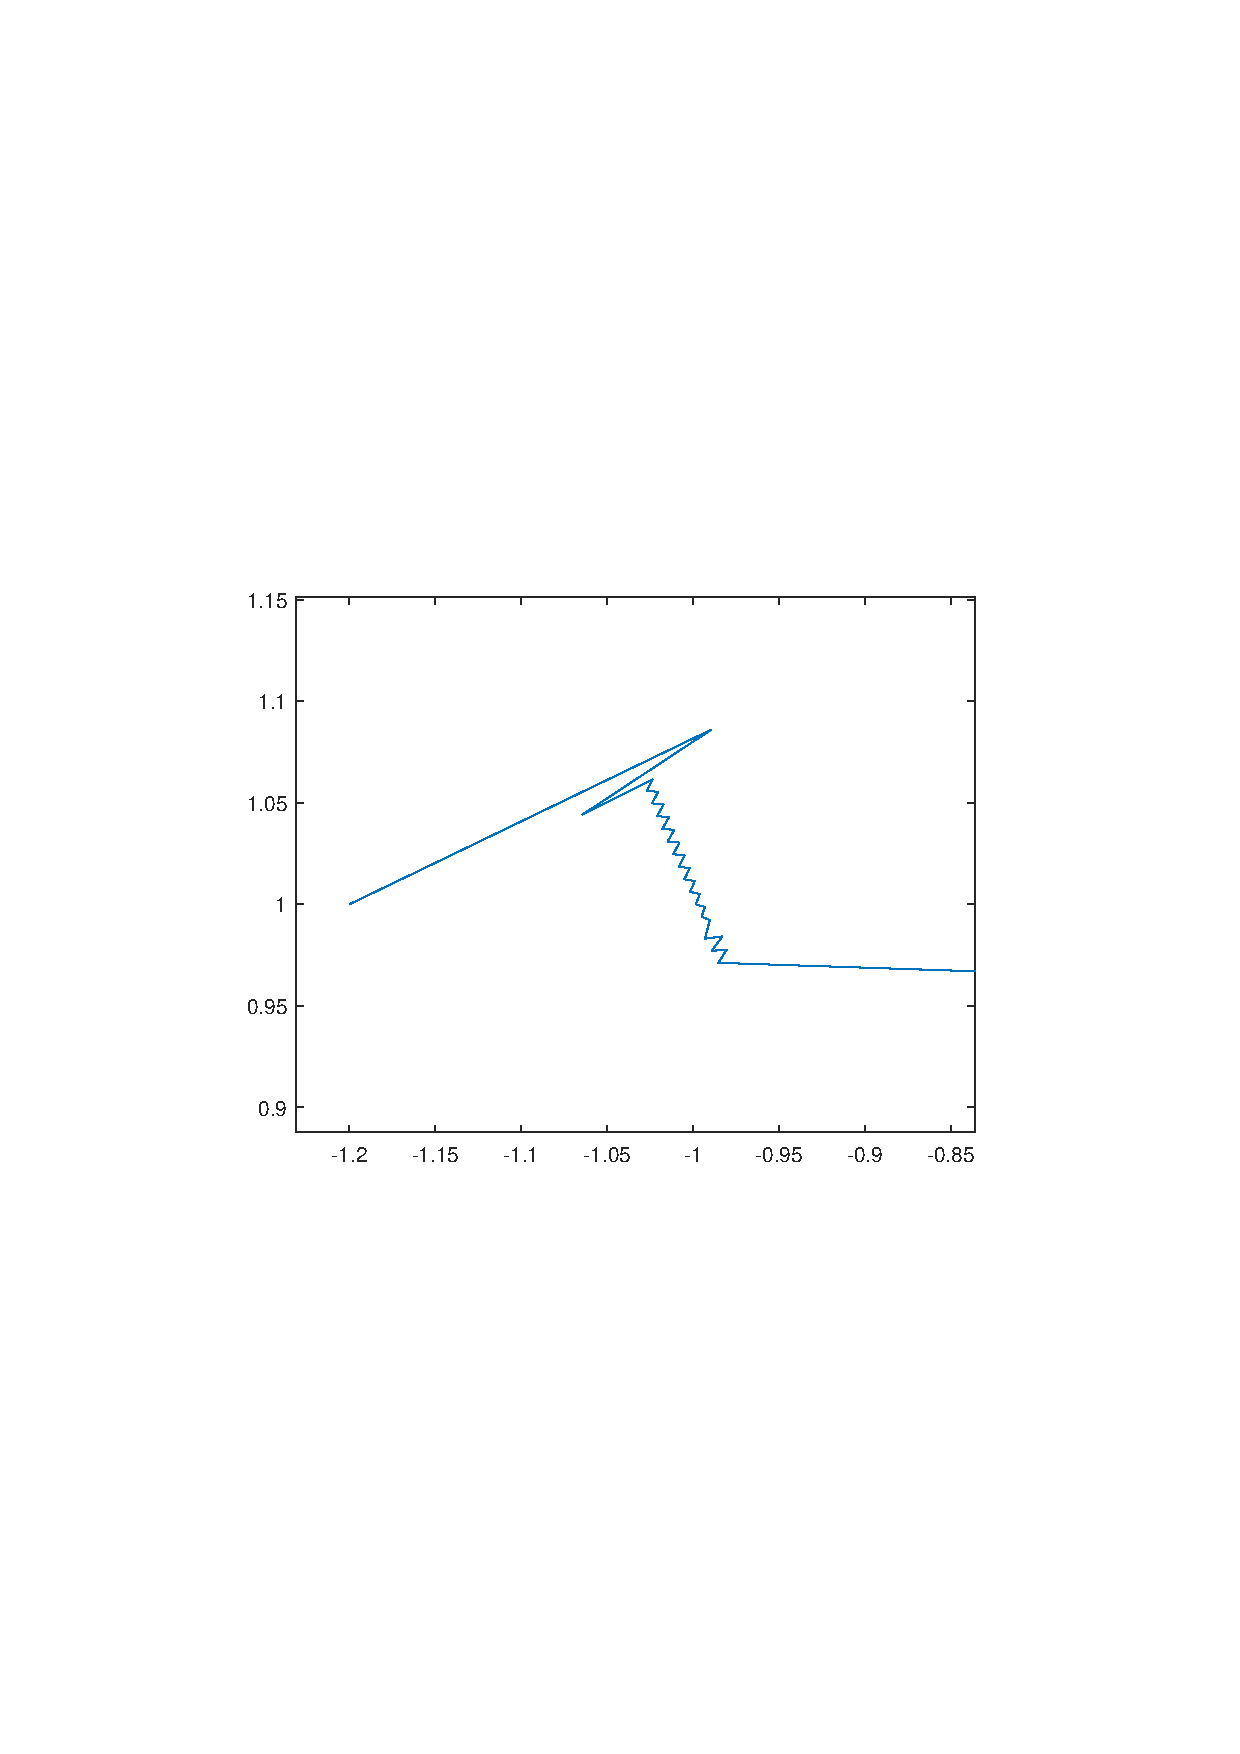
\includegraphics[width=5cm]{fig/4_22.pdf}}
\subfigure{
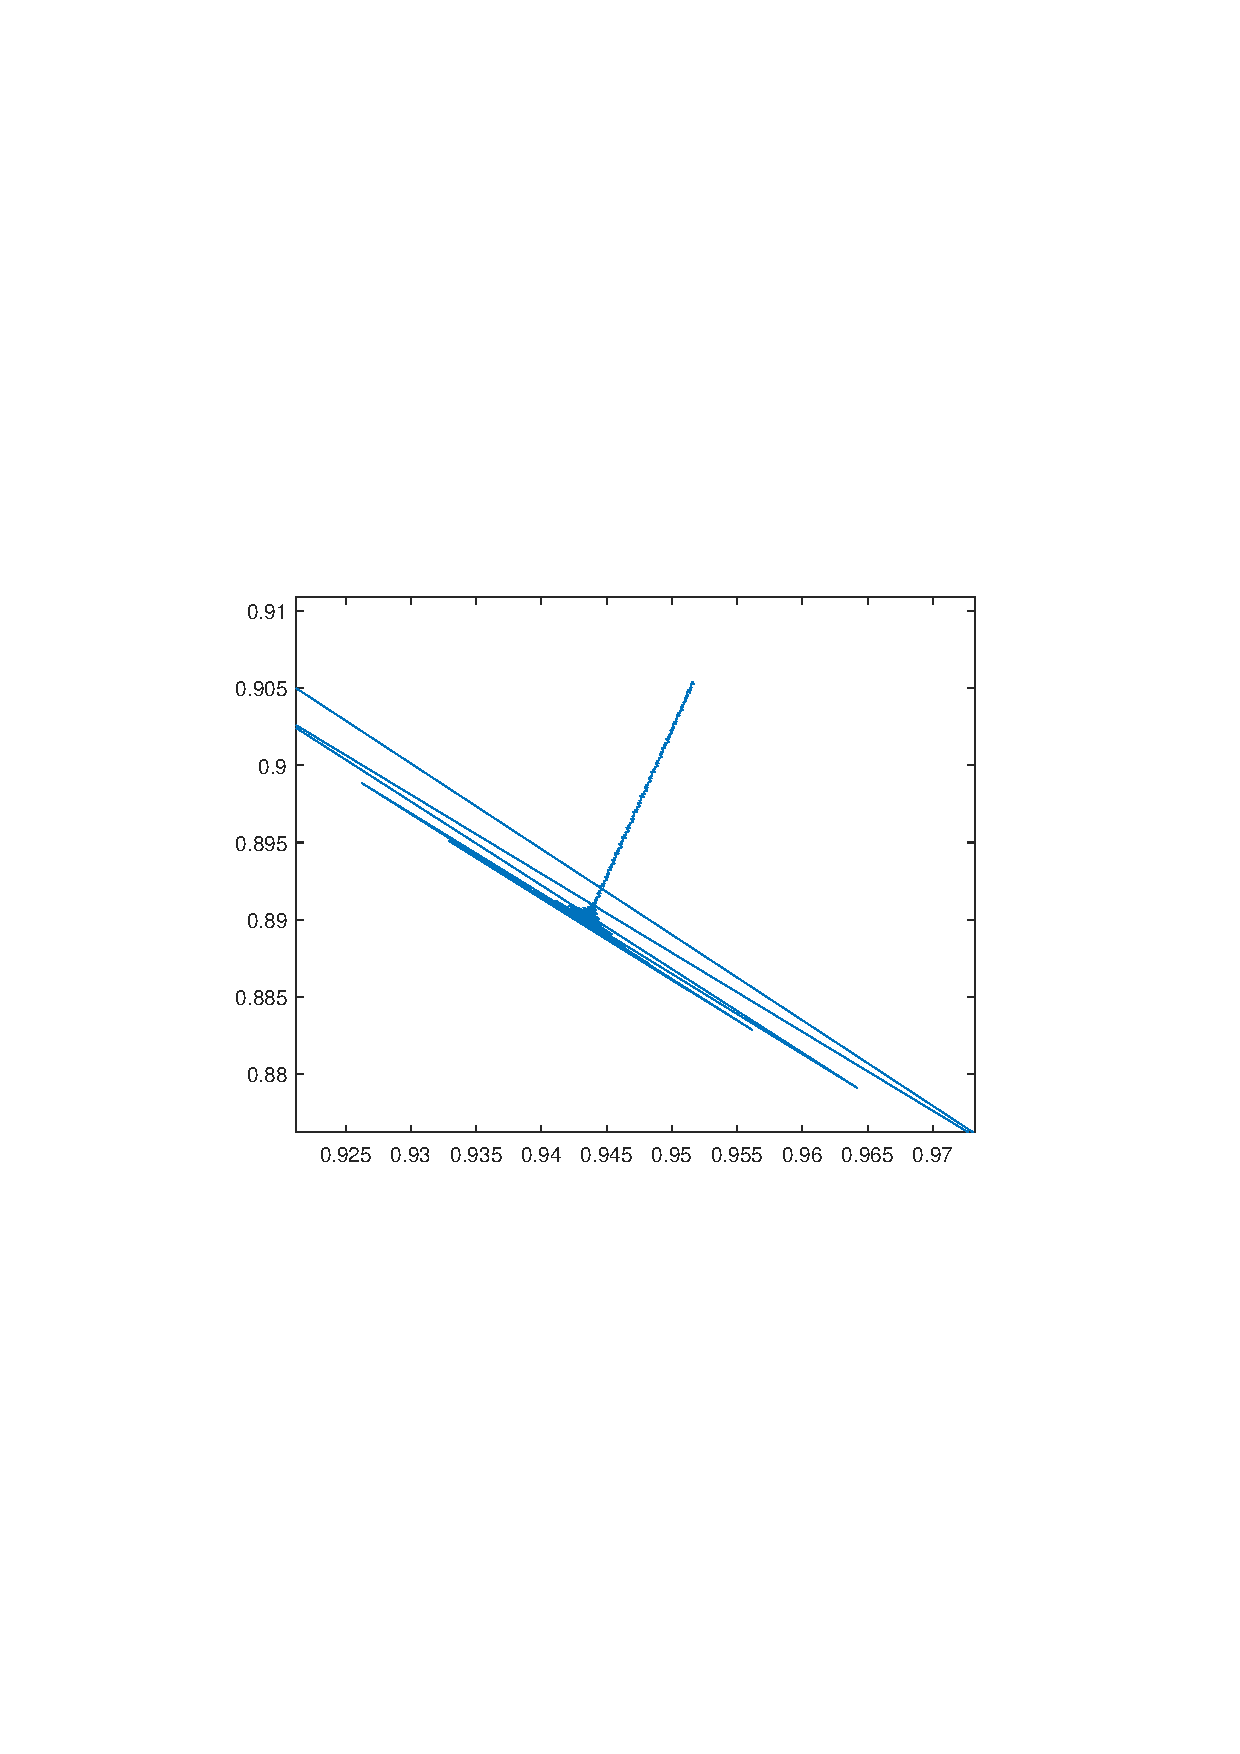
\includegraphics[width=5cm]{fig/4_23.pdf}}
\subfigure{
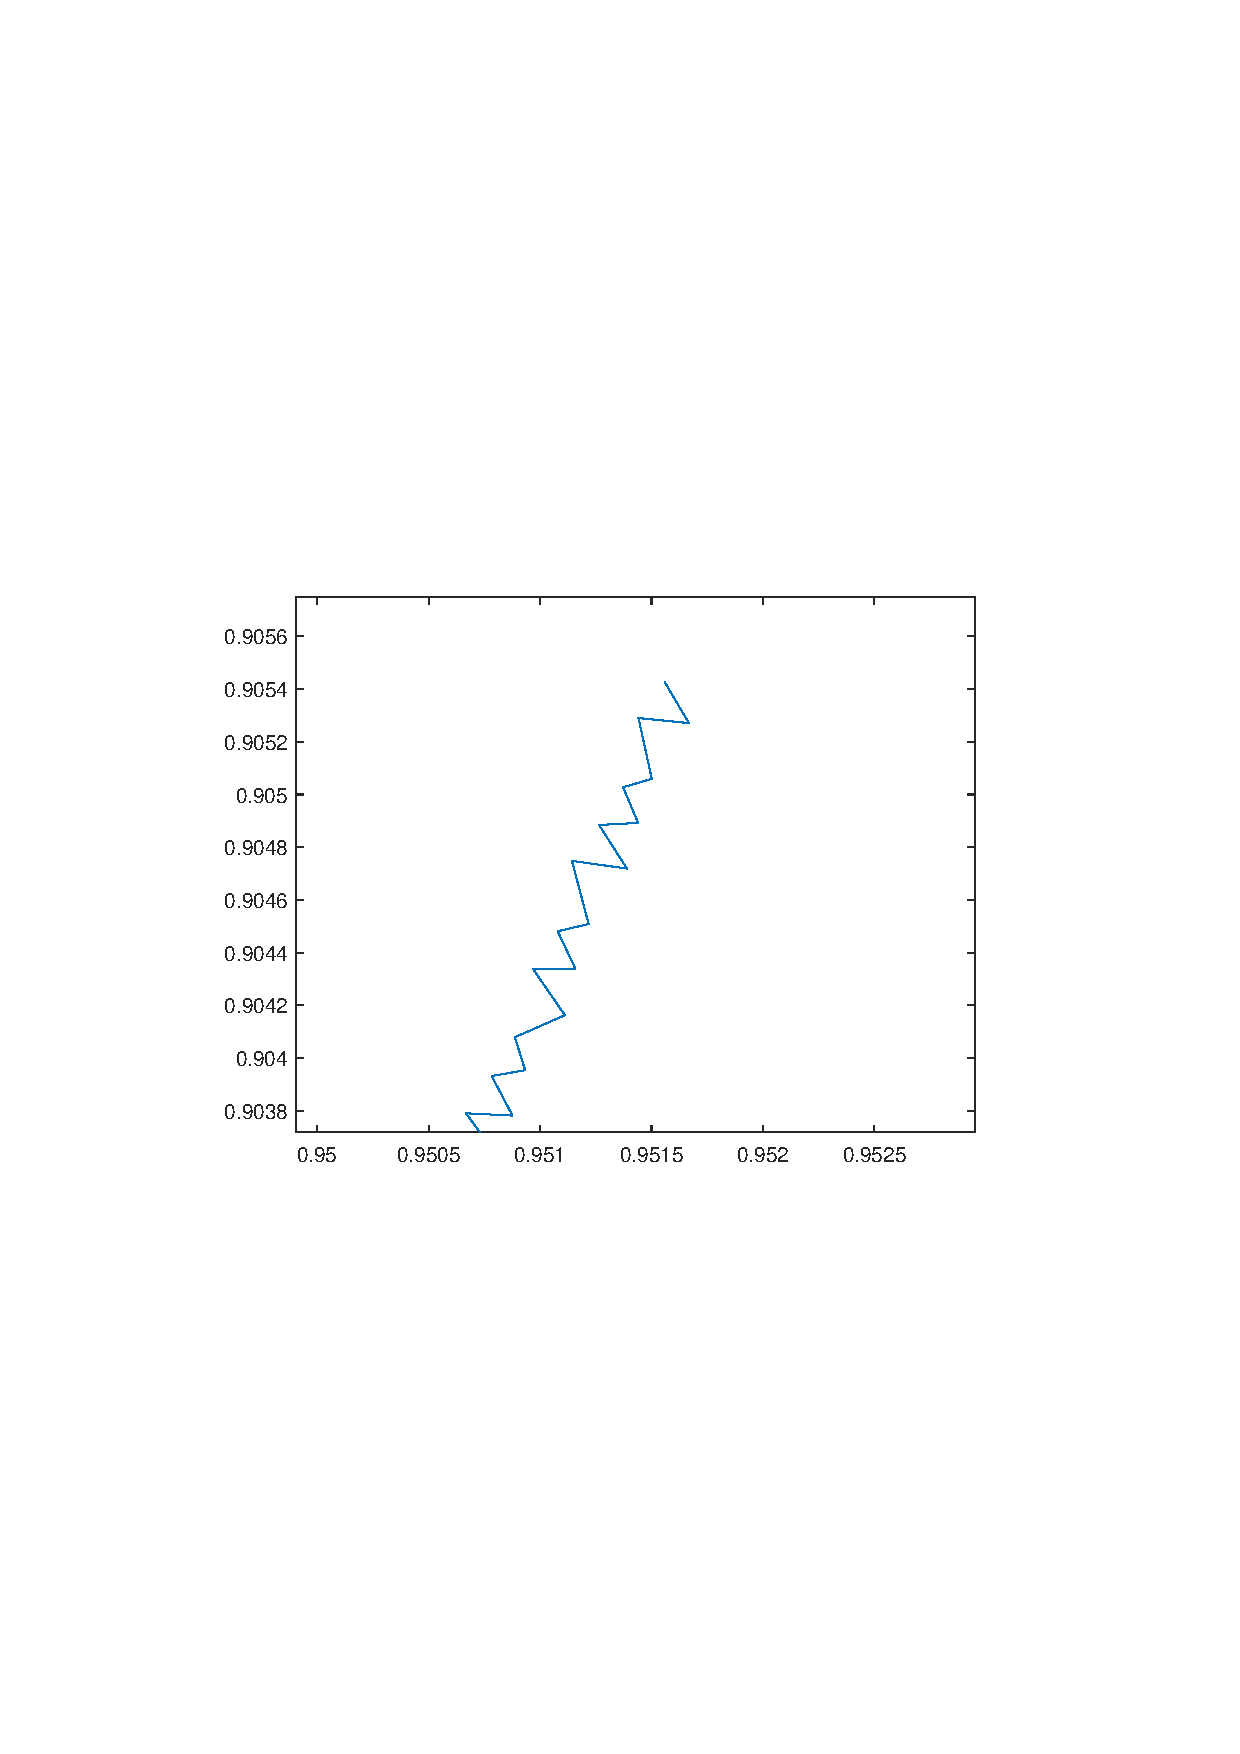
\includegraphics[width=5cm]{fig/4_24.pdf}}
\caption{Steepest-denscent in (-1.2,1)}
\label{Fig.lable}
\end{figure}

\begin{figure}[H]
\centering
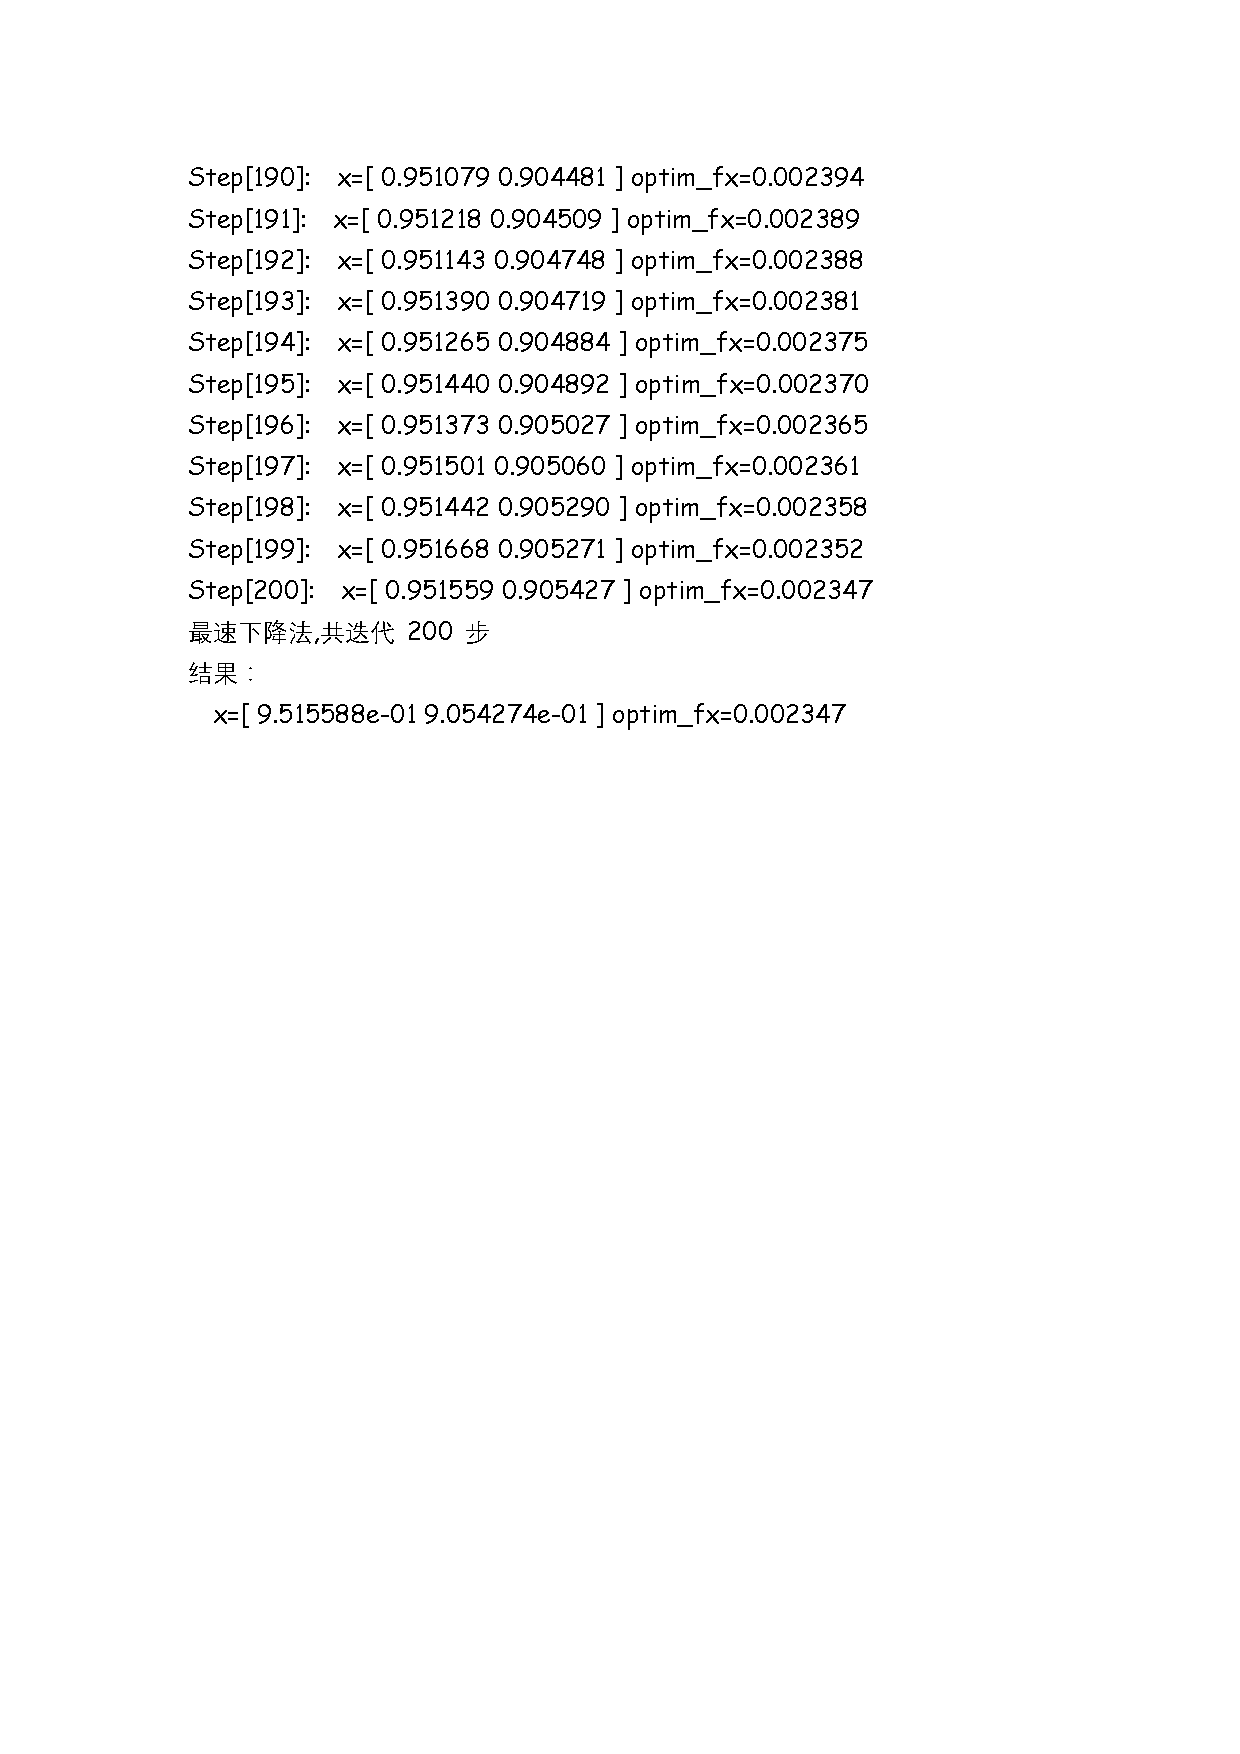
\includegraphics[width=10cm]{fig/4_25.pdf}
%\caption{在$(1,1)$处附近的三维等高线}
\end{figure}

\begin{figure}[H]
\centering
\subfigure{
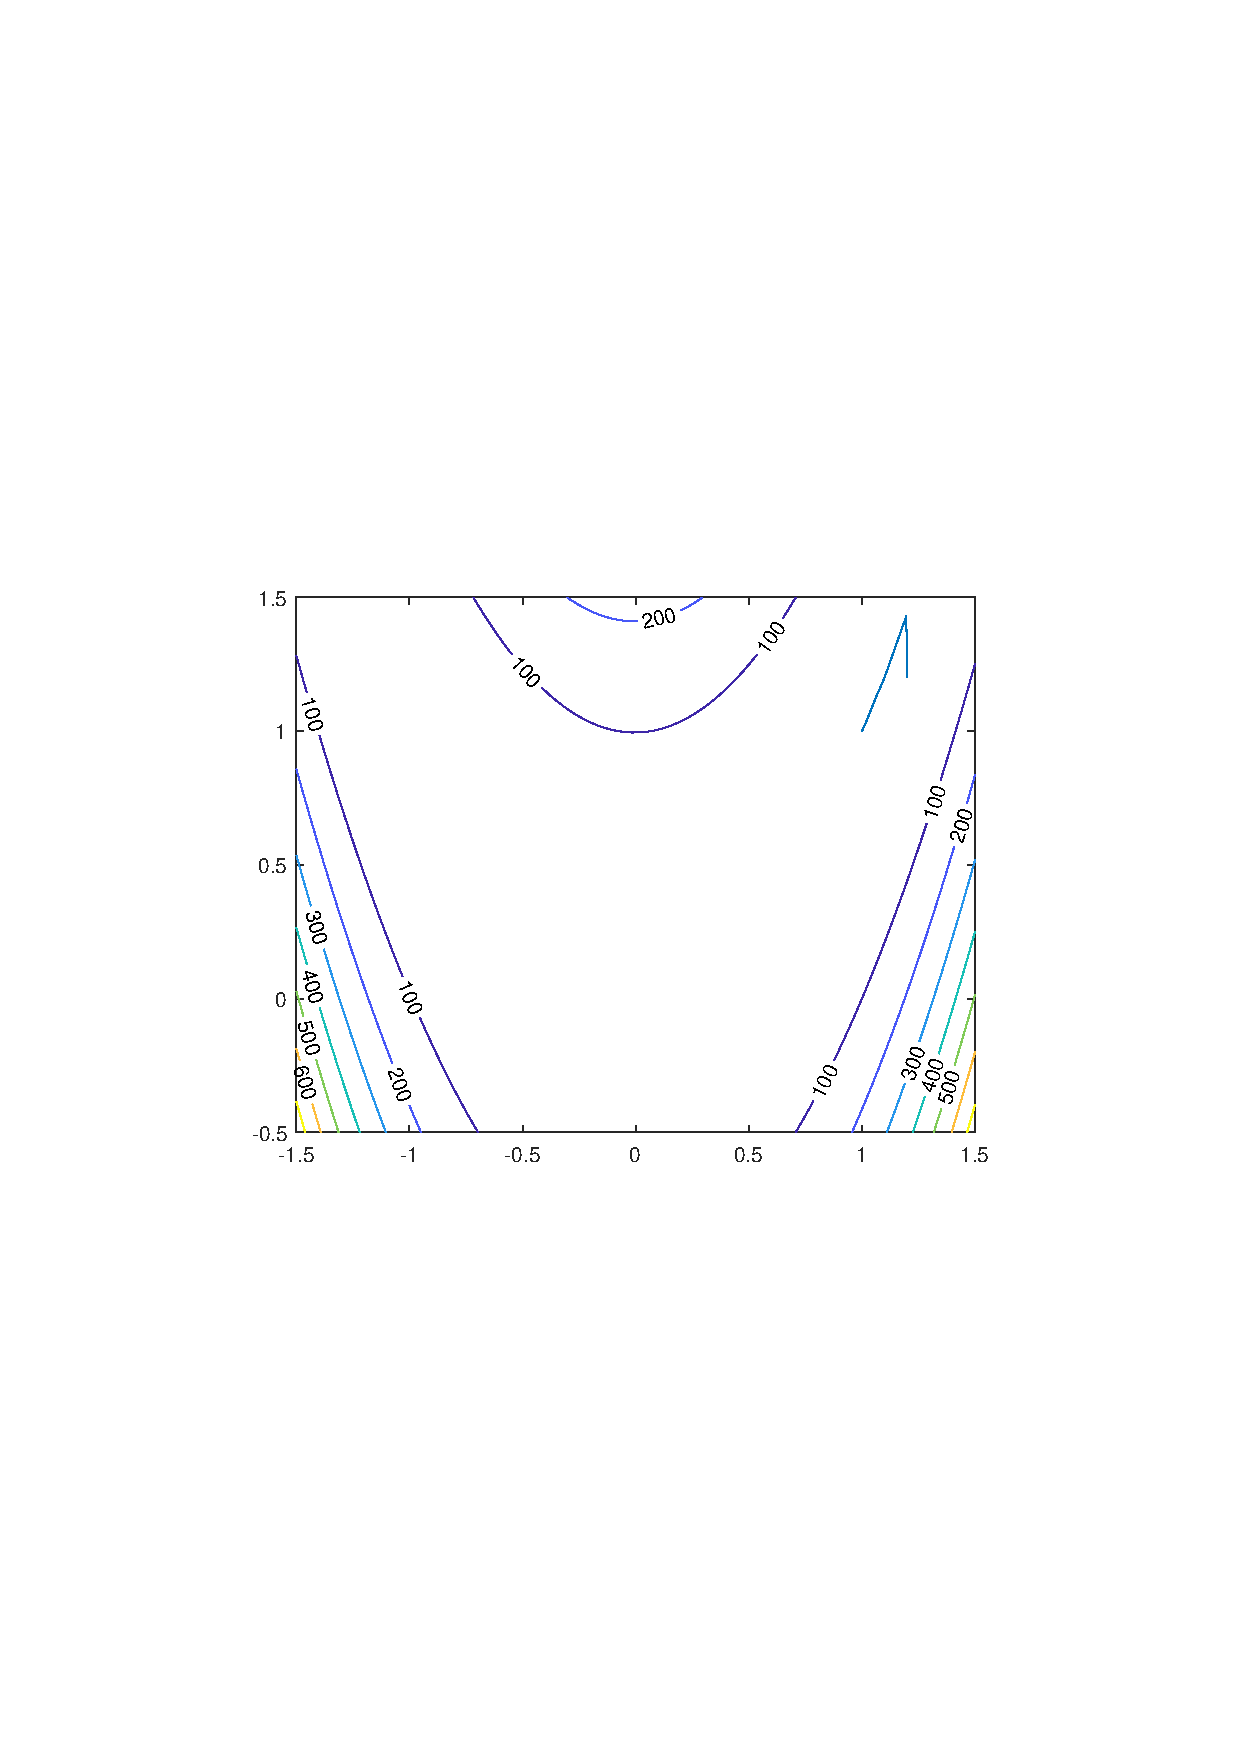
\includegraphics[width=5cm]{fig/4_31.pdf}}
\subfigure{
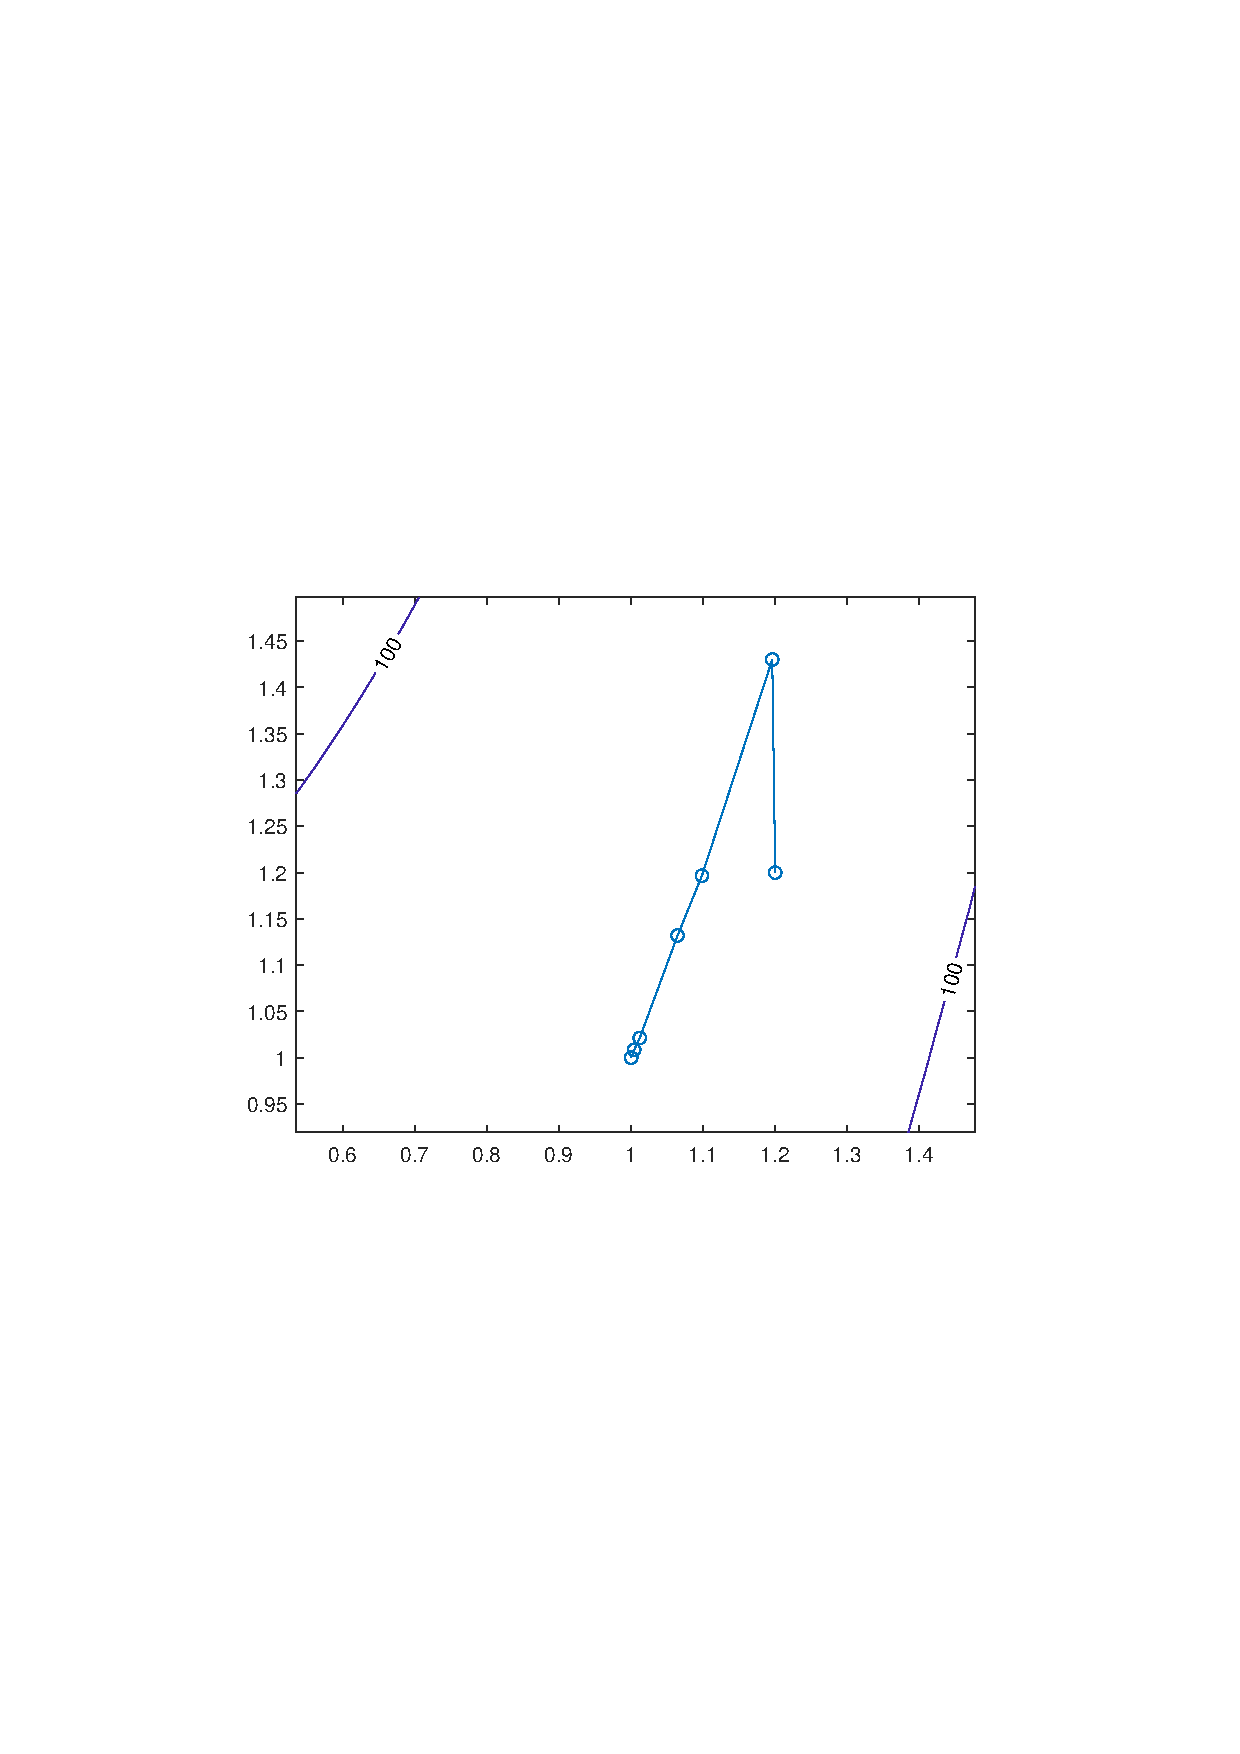
\includegraphics[width=5cm]{fig/4_32.pdf}}
\subfigure{
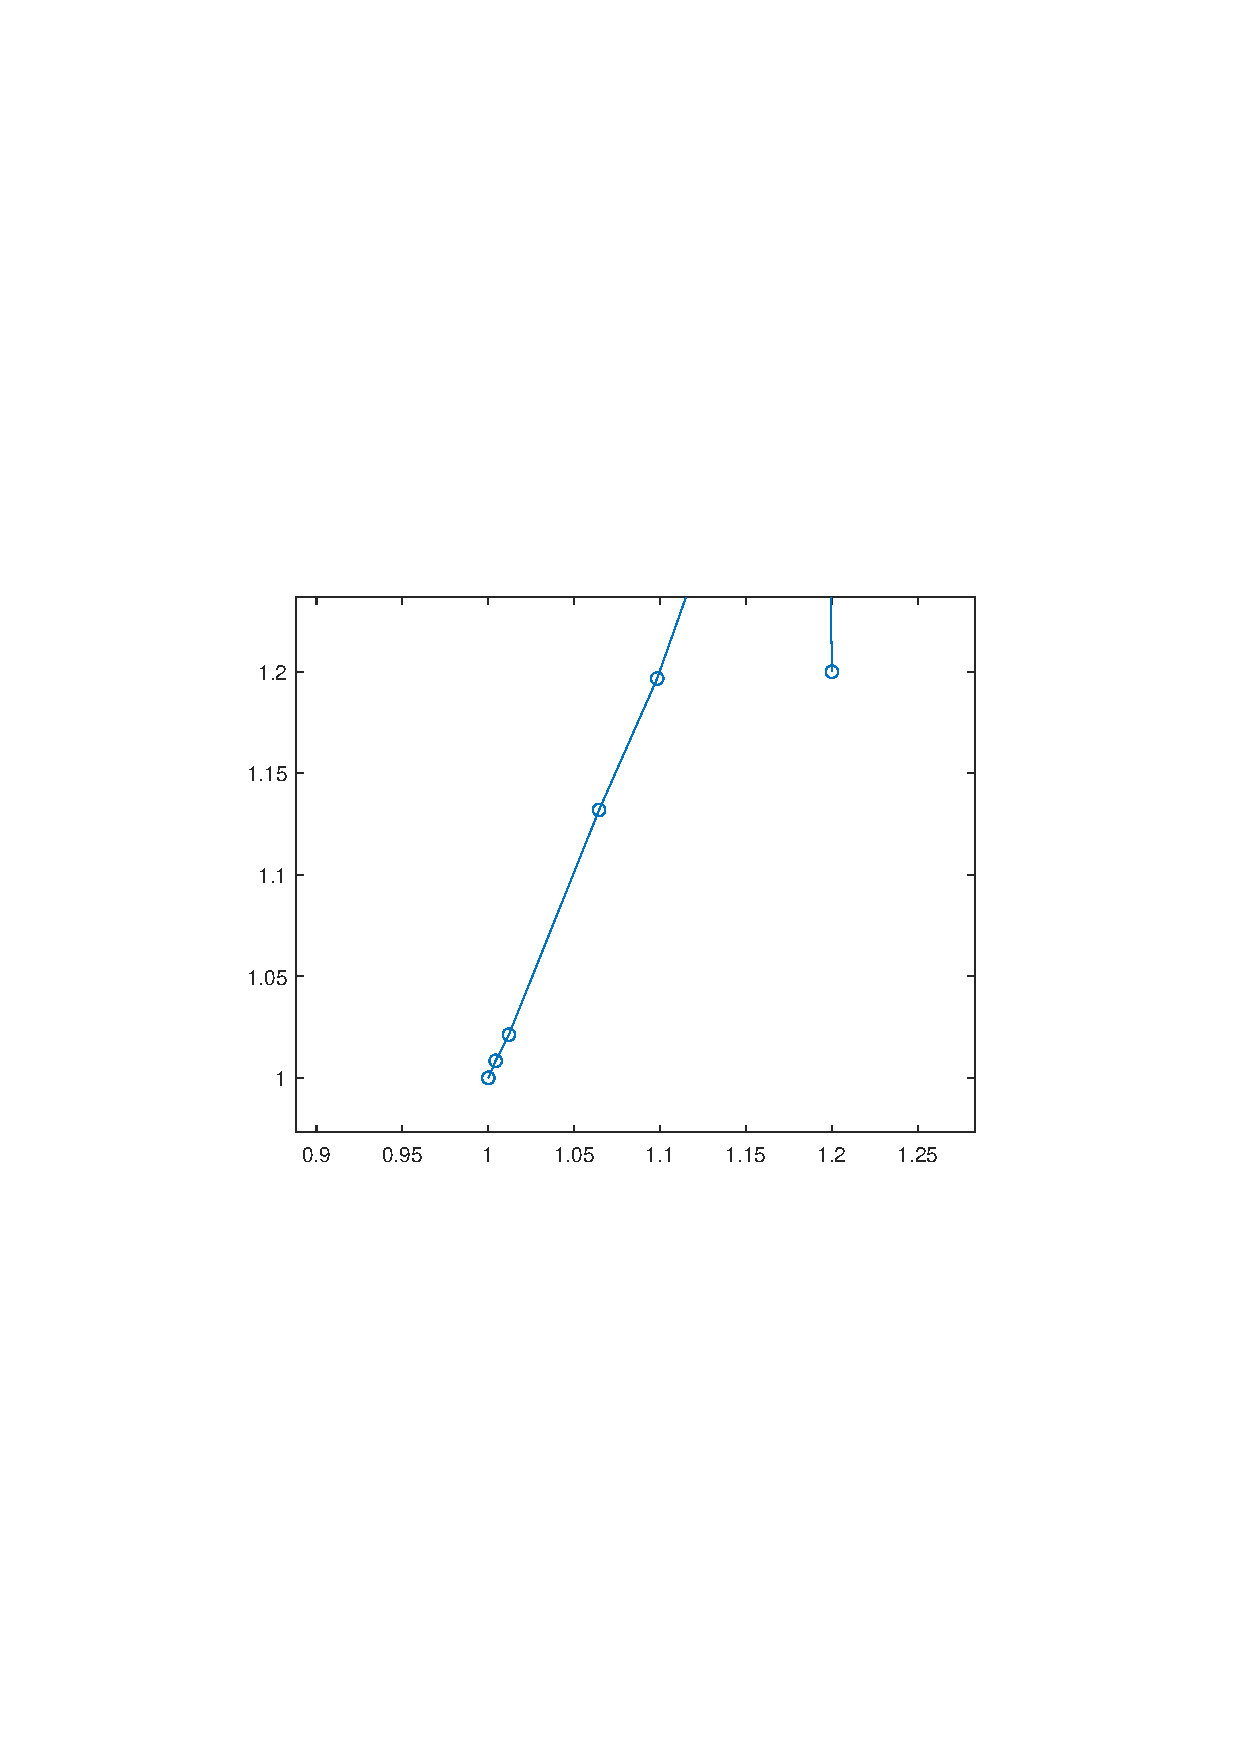
\includegraphics[width=5cm]{fig/4_33.pdf}}
\subfigure{
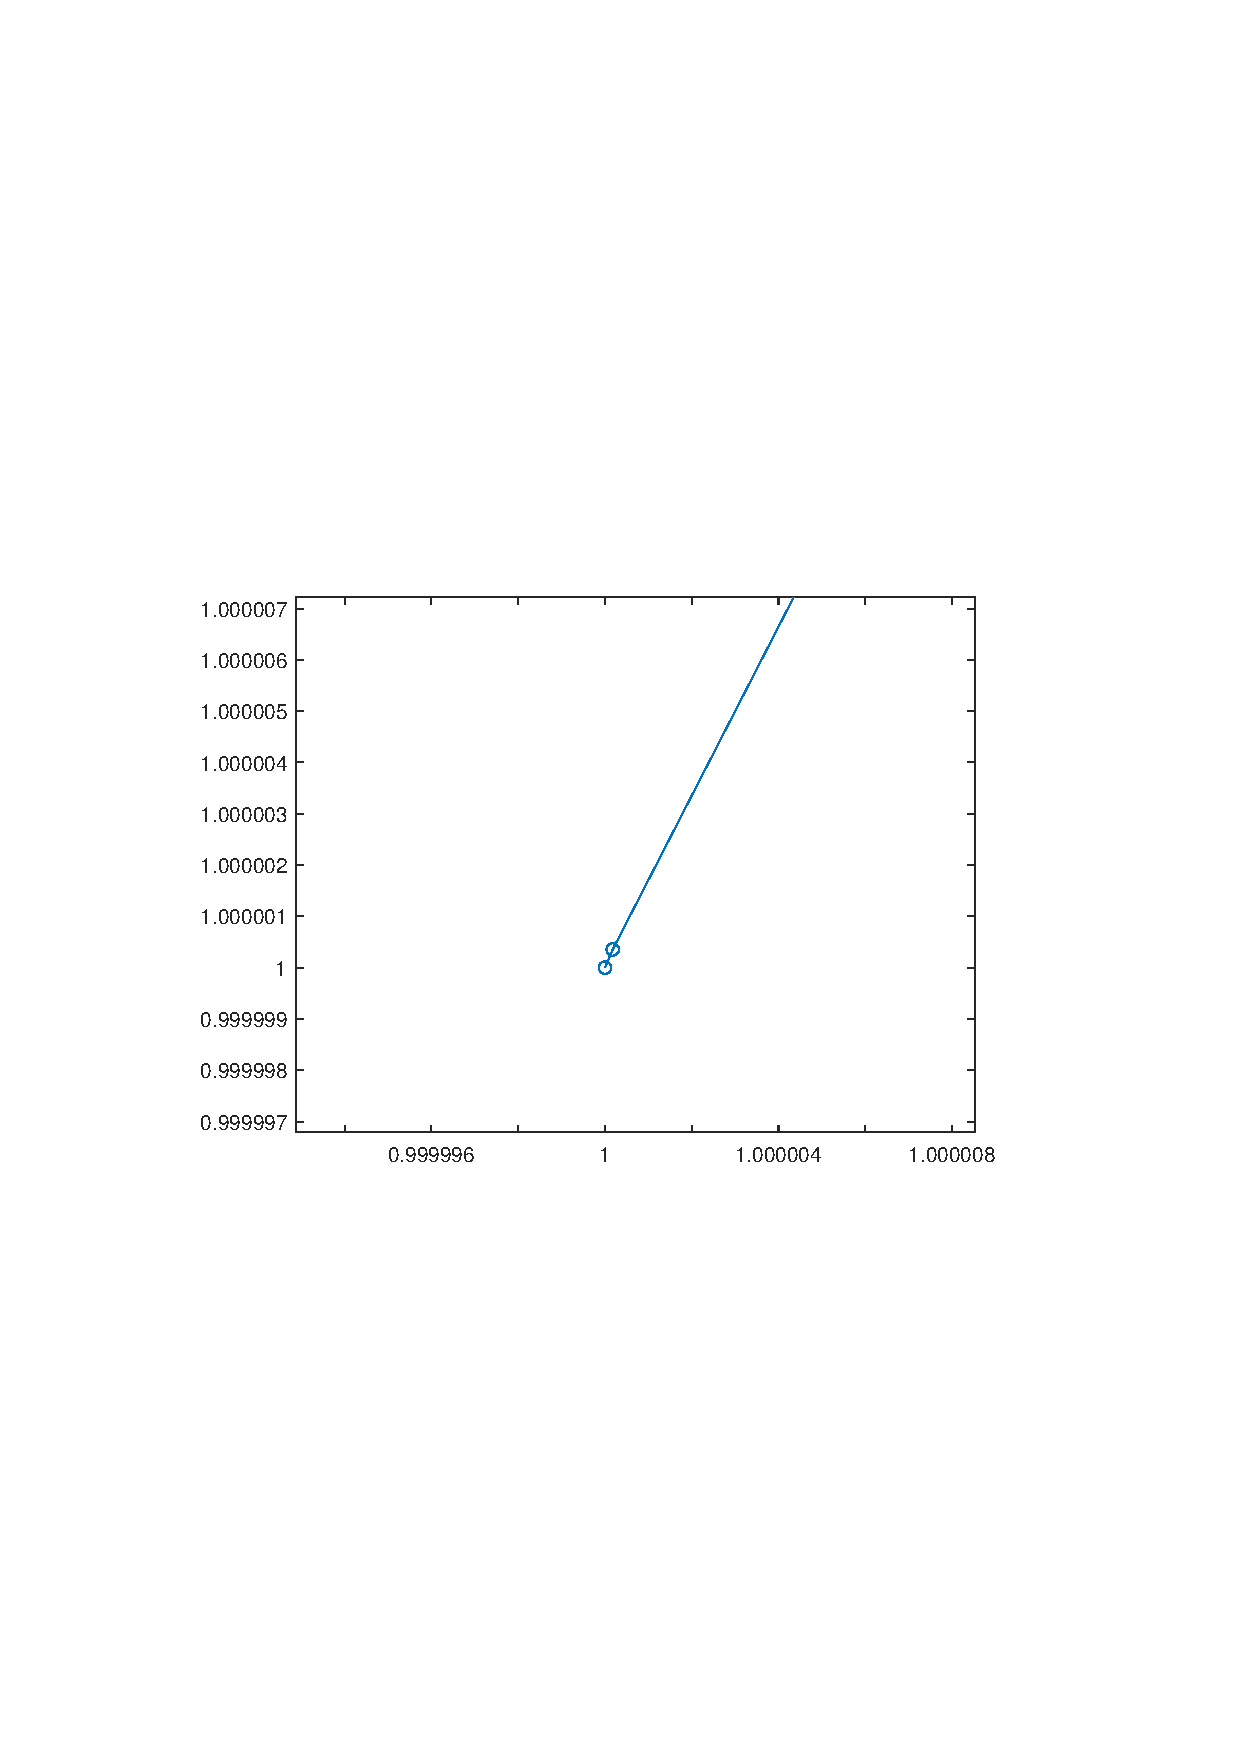
\includegraphics[width=5.3cm]{fig/4_34.pdf}}
\caption{Newton-Armijo in (1.2,1.2)}
\label{Fig.lable}
\end{figure}

\begin{figure}[H]
\centering
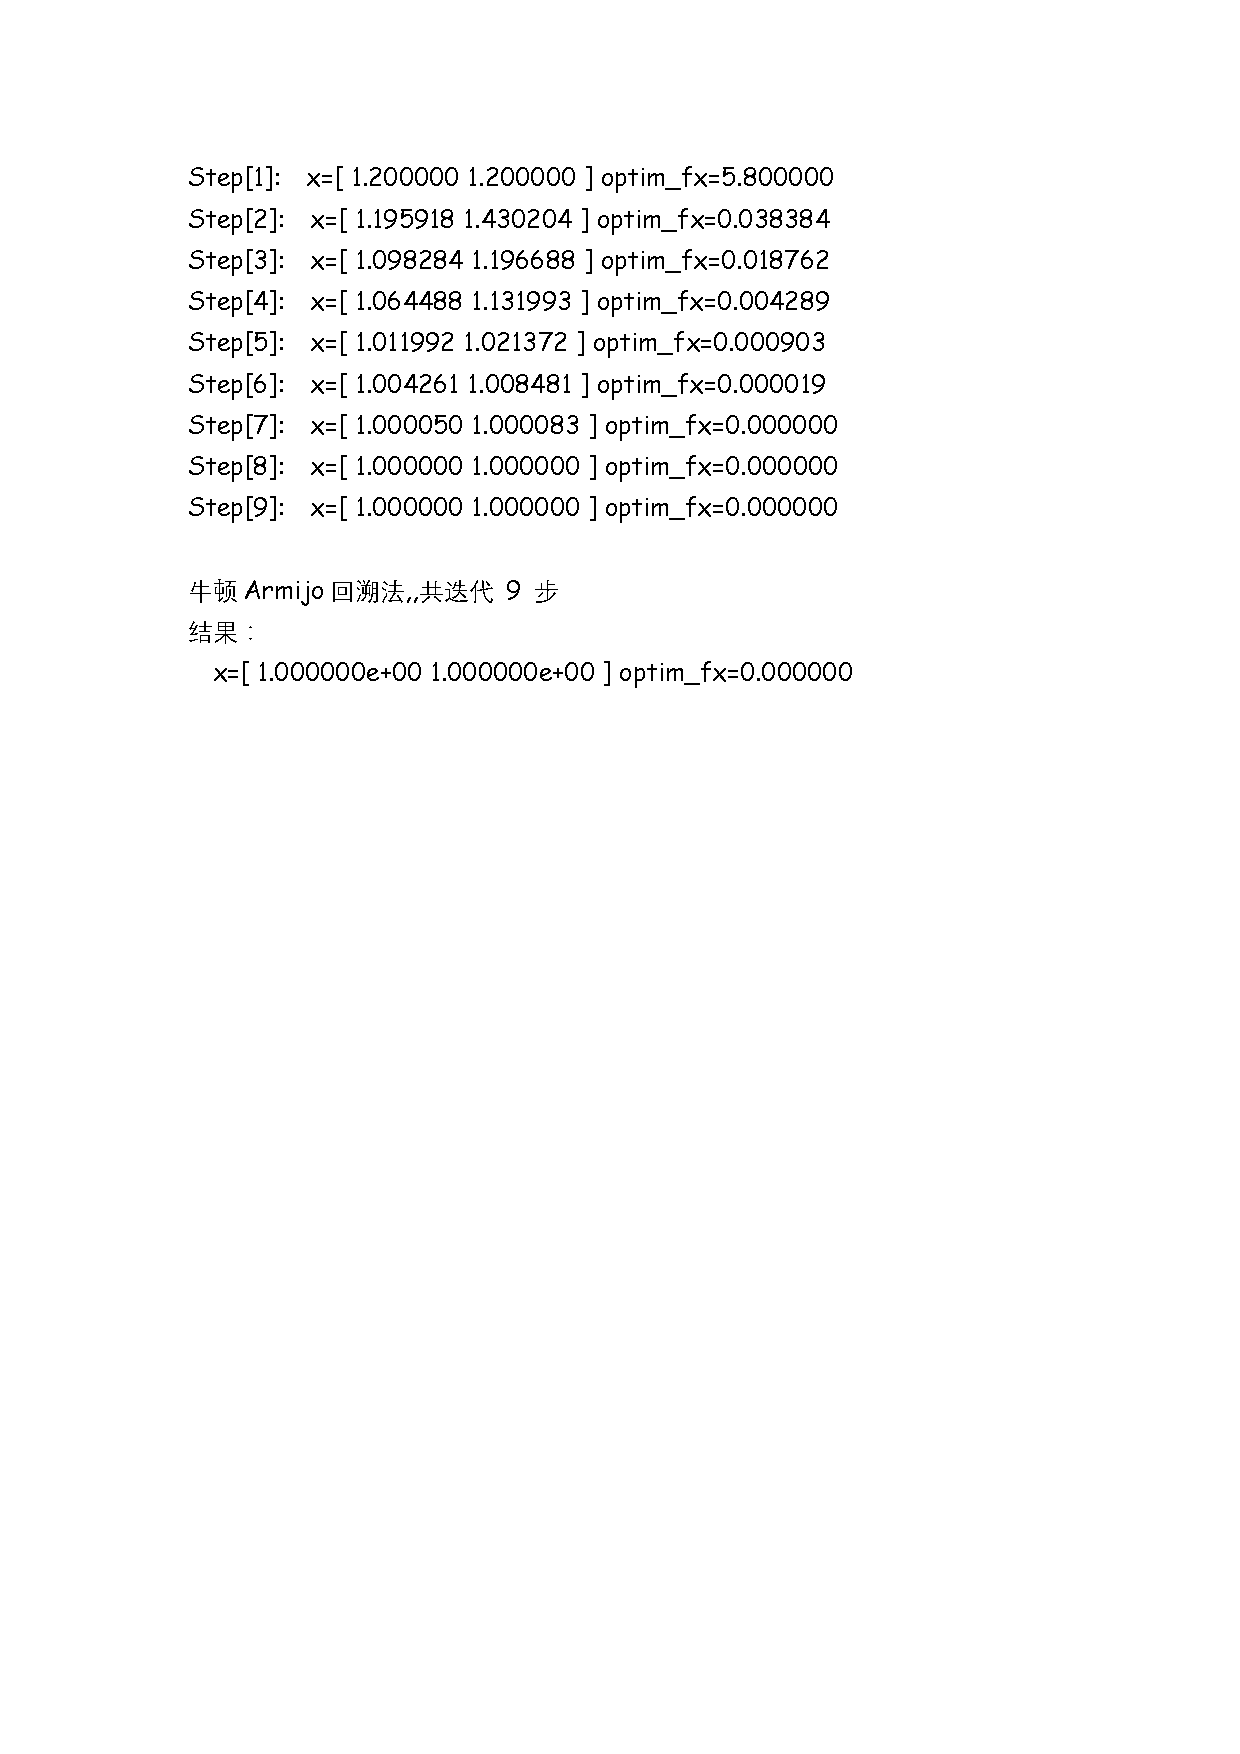
\includegraphics[width=10cm]{fig/4_35.pdf}
%\caption{在$(1,1)$处附近的三维等高线}
\end{figure}

\begin{figure}[H]
\centering
\subfigure{
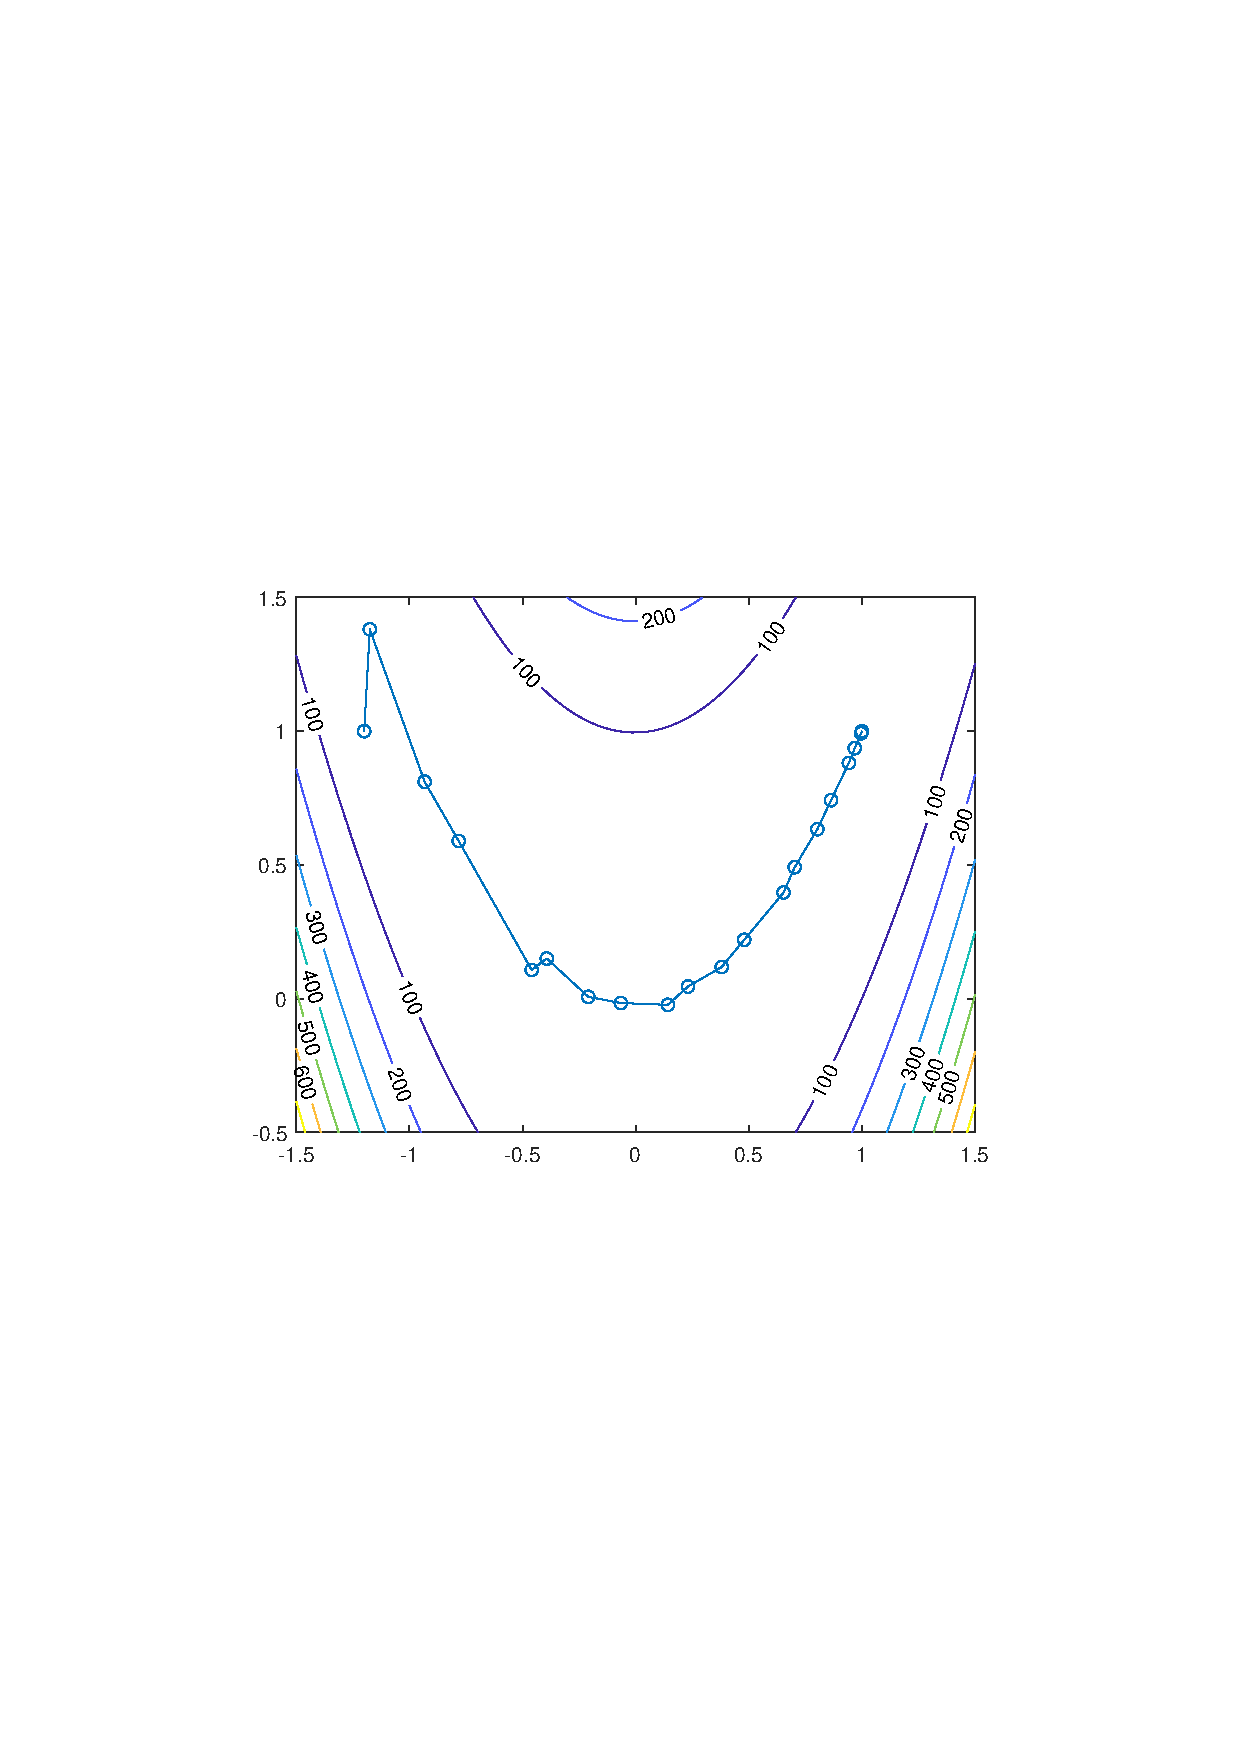
\includegraphics[width=5cm]{fig/4_41.pdf}}
\subfigure{
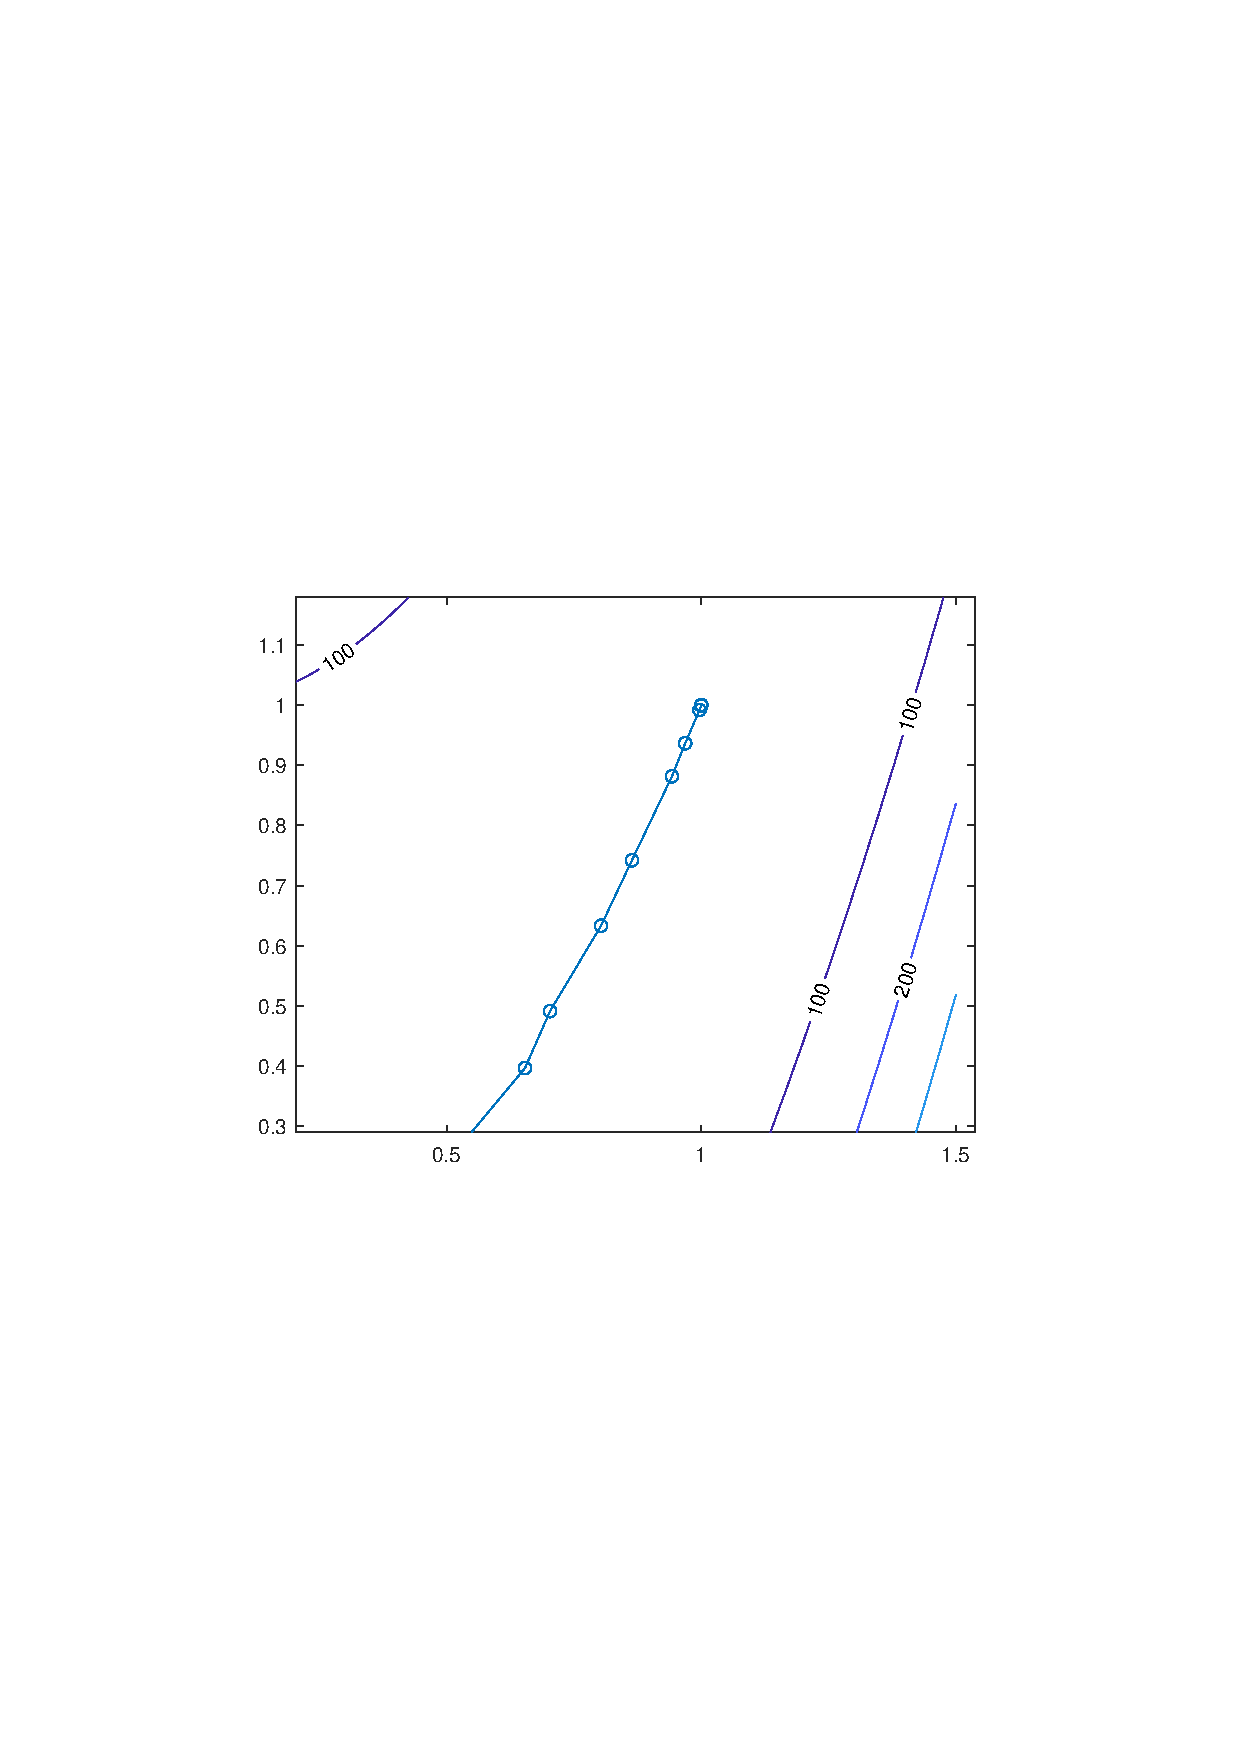
\includegraphics[width=5cm]{fig/4_42.pdf}}
\subfigure{
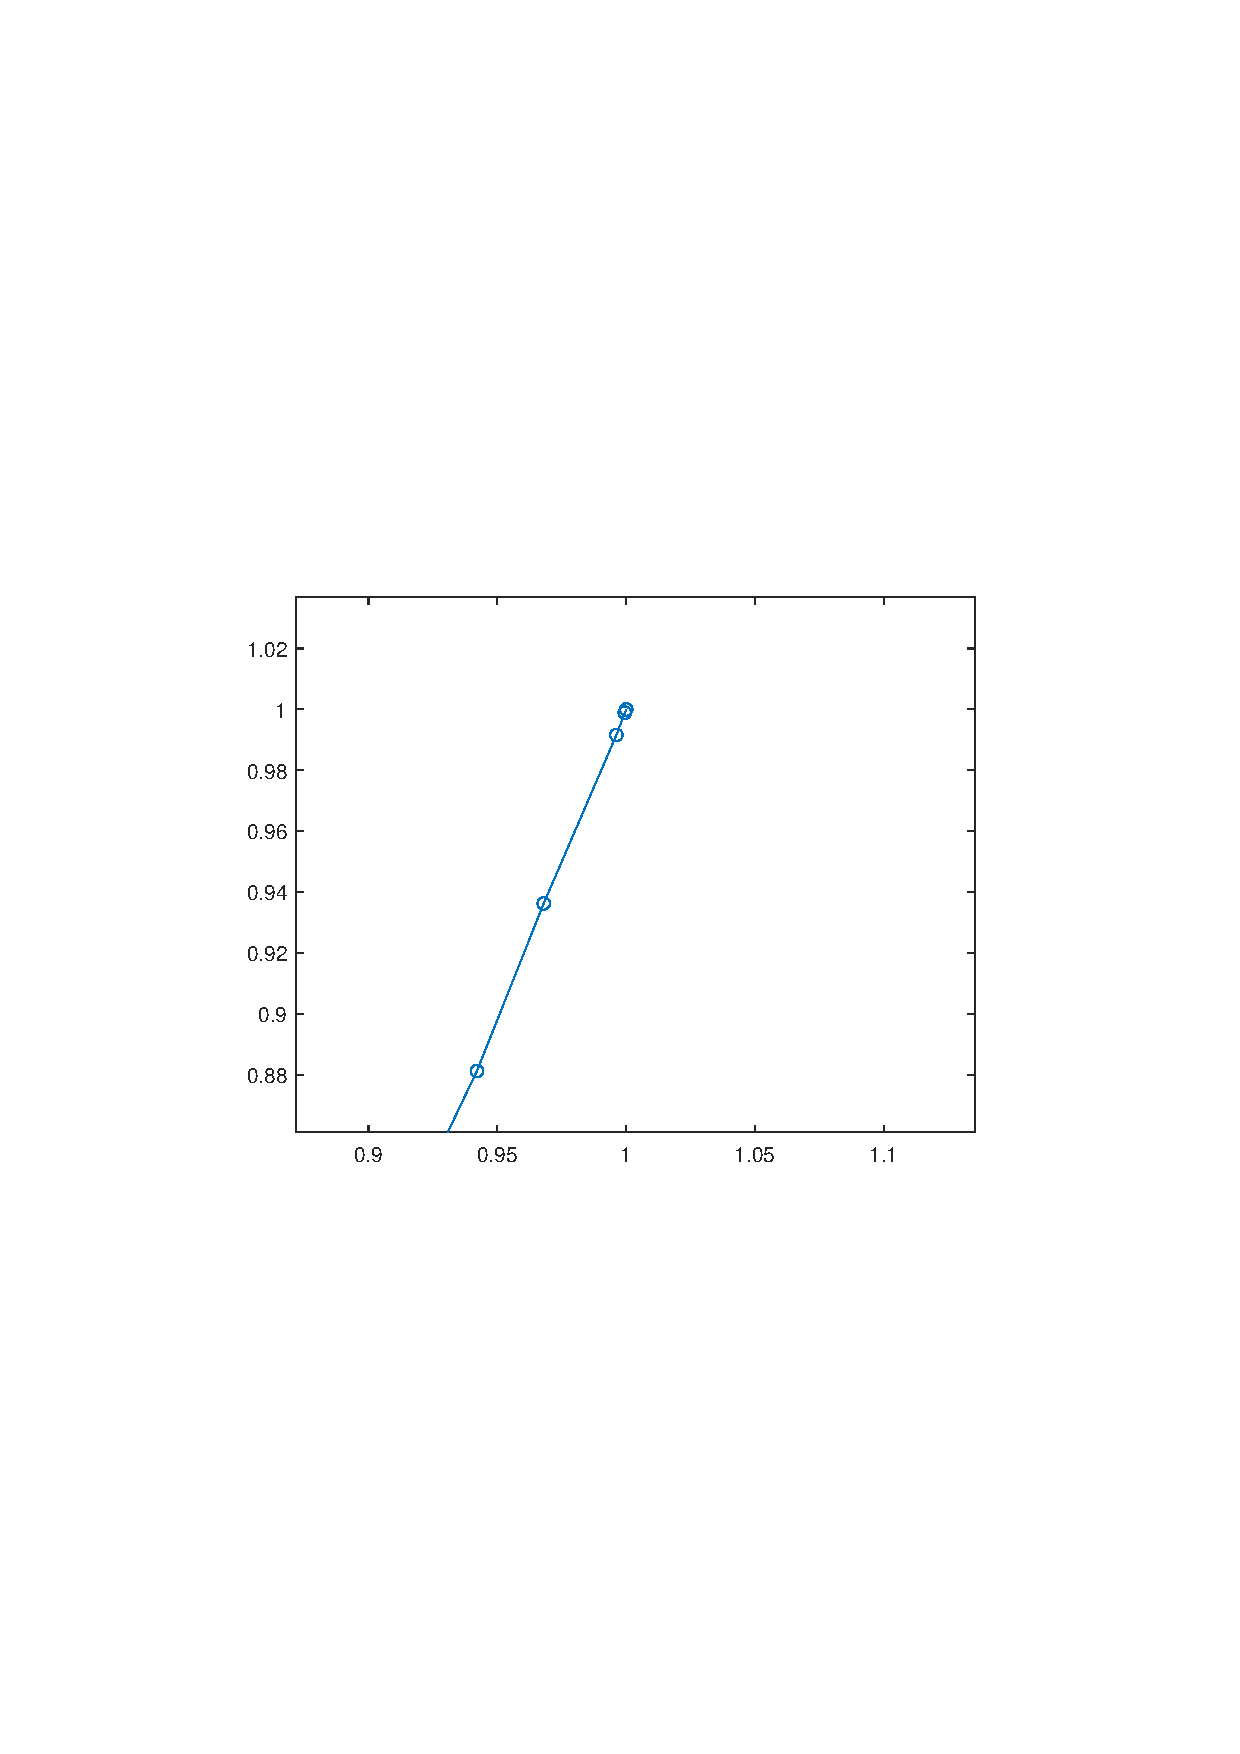
\includegraphics[width=5cm]{fig/4_43.pdf}}
\subfigure{
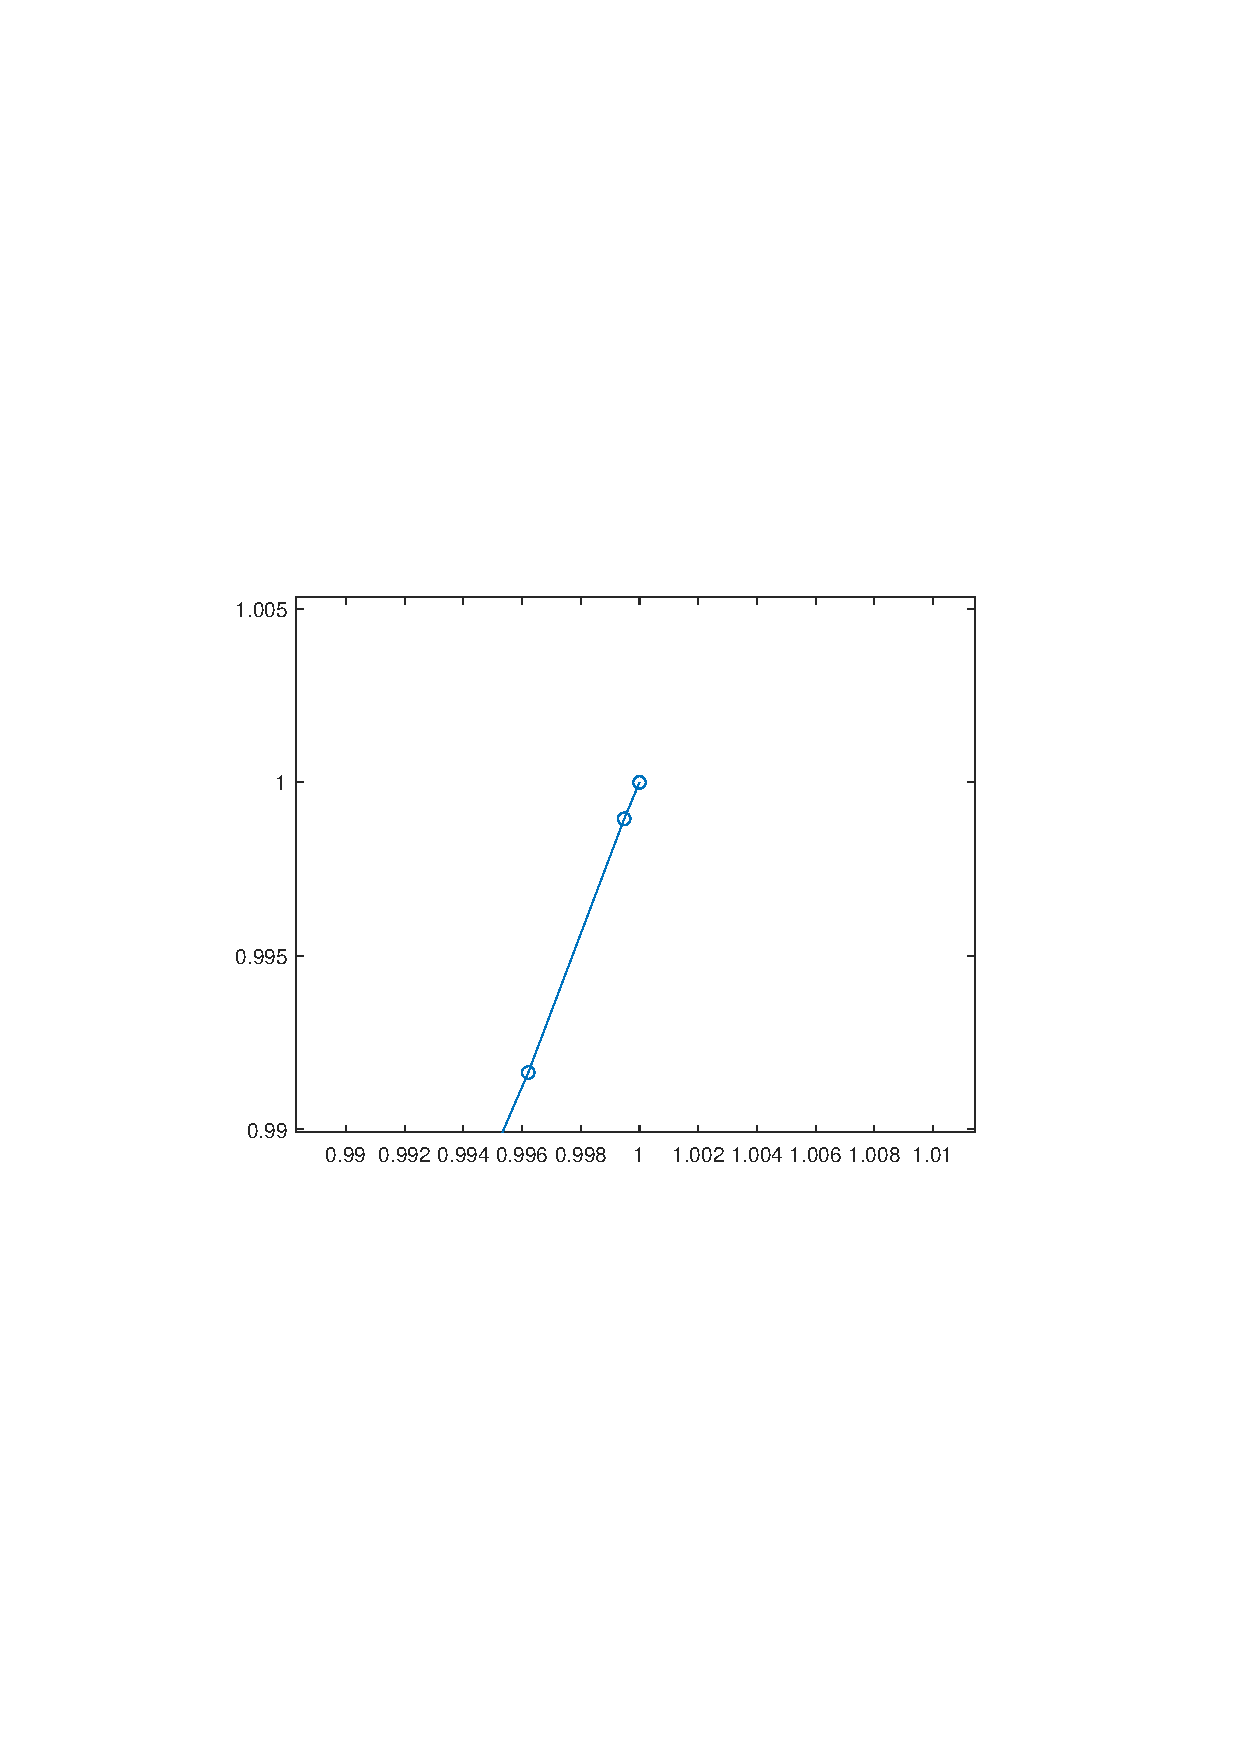
\includegraphics[width=5.3cm]{fig/4_44.pdf}}
\caption{Newton-Armijo in (-1.2,1)}
\label{Fig.lable}
\end{figure}

\begin{figure}[H]
\centering
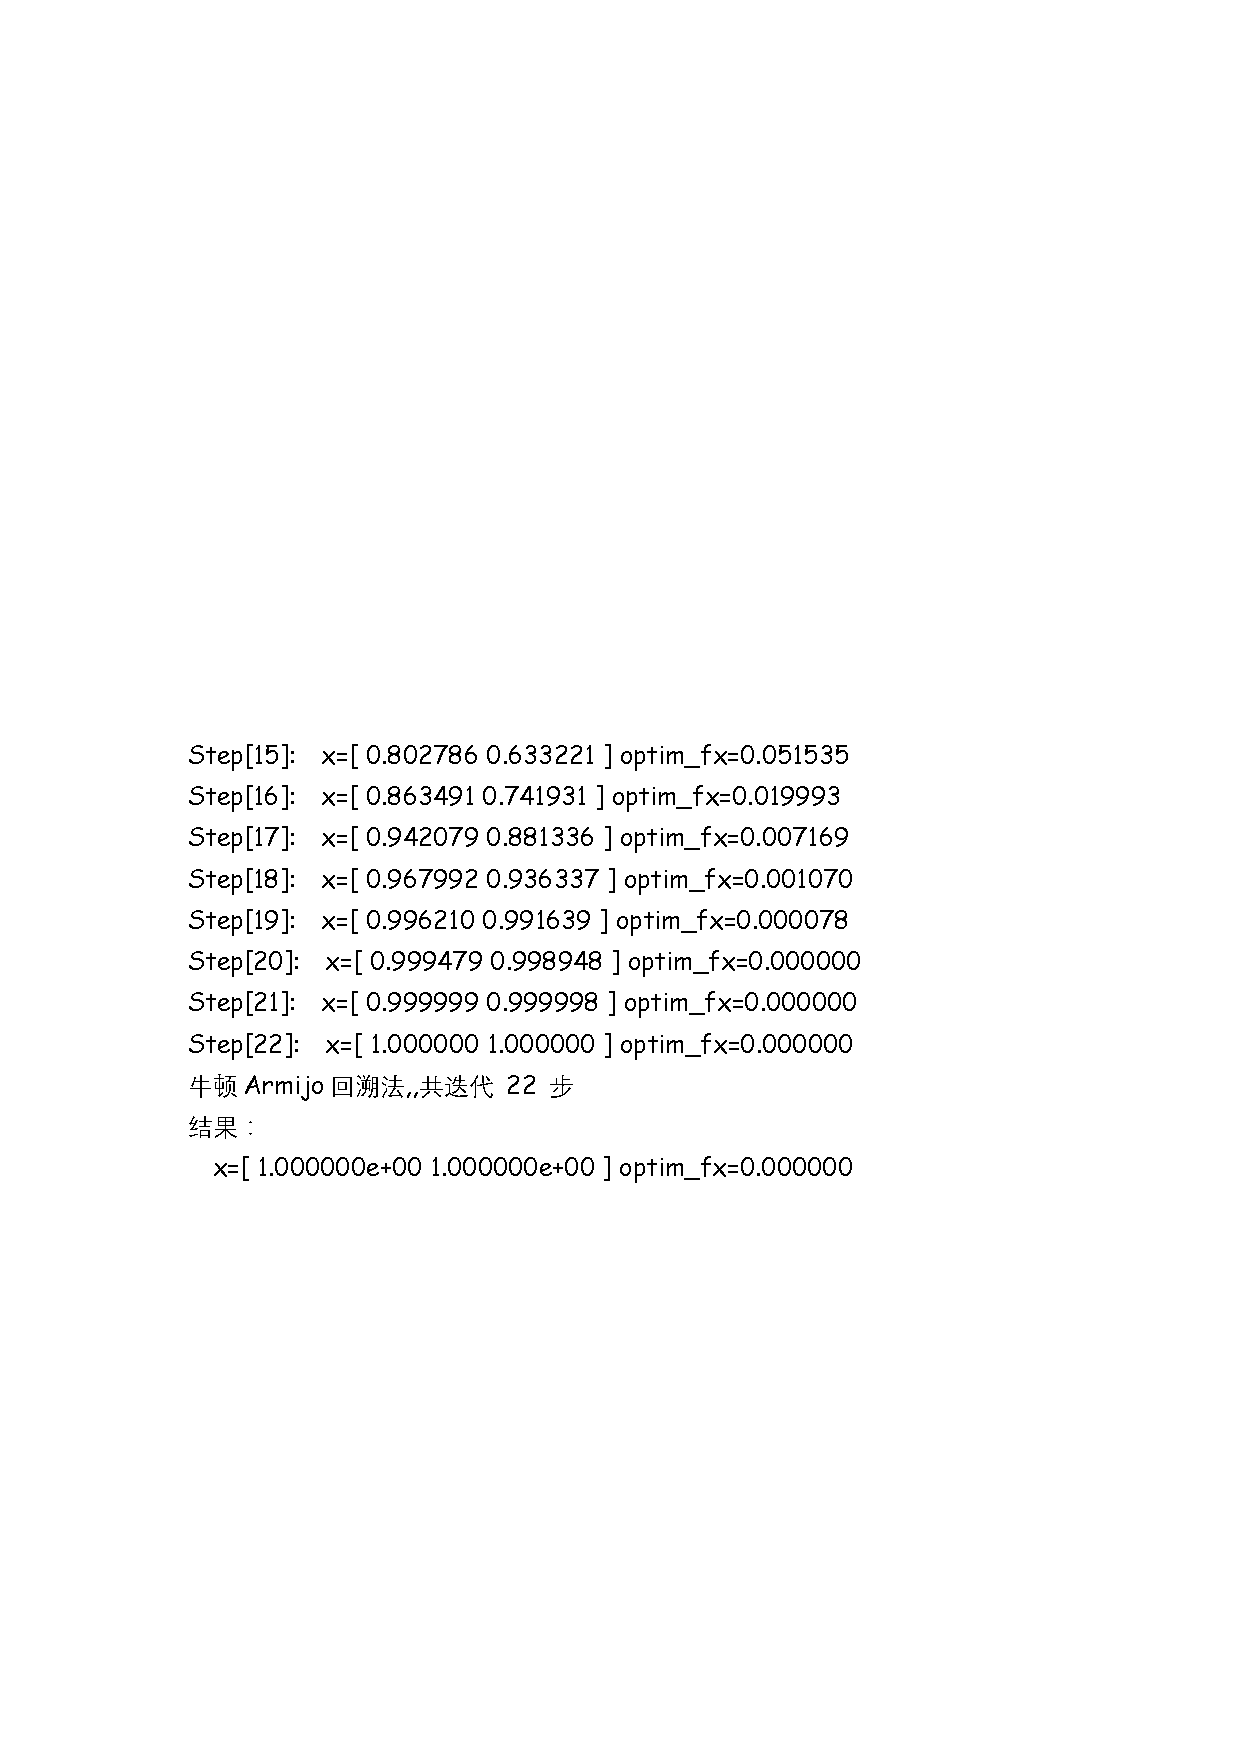
\includegraphics[width=10cm]{fig/4_45.pdf}
%\caption{在$(1,1)$处附近的三维等高线}
\end{figure}